% Customizable fields and text areas start with % >> below.
% Lines starting with the comment character (%) are normally removed before release outside the collaboration, but not those comments ending lines

% svn info. These are modified by svn at checkout time.
% The last version of these macros found before the maketitle will be the one on the front page,
% so only the main file is tracked.
% Do not edit by hand!
\RCS$Revision: 404452 $
\RCS$HeadURL: svn+ssh://svn.cern.ch/reps/tdr2/notes/HIG-17-005/trunk/HIG-17-005.tex $
\RCS$Id: HIG-17-005.tex 404452 2017-05-12 20:53:41Z stiegerb $
%%%%%%%%%%%%% local definitions %%%%%%%%%%%%%%%%%%%%%
% This allows for switching between one column and two column (cms@external) layouts
% The widths should  be modified for your particular figures. You'll need additional copies if you have more than one standard figure size.
\newlength\cmsFigWidth
\ifthenelse{\boolean{cms@external}}{\setlength\cmsFigWidth{0.85\columnwidth}}{\setlength\cmsFigWidth{0.4\textwidth}}
\ifthenelse{\boolean{cms@external}}{\providecommand{\cmsLeft}{top\xspace}}{\providecommand{\cmsLeft}{left\xspace}}
\ifthenelse{\boolean{cms@external}}{\providecommand{\cmsRight}{bottom\xspace}}{\providecommand{\cmsRight}{right\xspace}}

\newcommand{\W}{\ensuremath{\cmsSymbolFace{W}}\xspace}
\newcommand{\ZZ}{\ensuremath{\cmsSymbolFace{ZZ}}\xspace}
\newcommand{\WW}{\ensuremath{\cmsSymbolFace{WW}}\xspace}
\newcommand{\WZ}{\ensuremath{\cmsSymbolFace{WZ}}\xspace}
\newcommand{\VVV}{\ensuremath{\cmsSymbolFace{VVV}}\xspace}
\newcommand{\WVV}{\ensuremath{\cmsSymbolFace{WVV}}\xspace}
\newcommand{\tautau}{\ensuremath{\Pgt\Pgt}\xspace}
\newcommand{\gaga}{\ensuremath{\Pgg\Pgg}\xspace}
\newcommand{\ttW}{\ensuremath{\ttbar\cmsSymbolFace{W}^{\pm}}\xspace}
\newcommand{\ttWW}{\ensuremath{\ttbar\WW}\xspace}
\newcommand{\ttZ}{\ensuremath{\ttbar\cmsSymbolFace{Z}}\xspace}
\newcommand{\ttH}{\ensuremath{\ttbar\cmsSymbolFace{H}}\xspace}
\newcommand{\ttG}{\ensuremath{\ttbar\gamma}\xspace}
\newcommand{\ttV}{\ensuremath{\ttbar\cmsSymbolFace{V}}\xspace}
\newcommand{\ttGStar}{\ensuremath{\ttbar\gamma^*}\xspace}
\newcommand{\tZq}{\ensuremath{\cPqt\Z\Pq}\xspace}
\newcommand{\WWqq}{\ensuremath{\W^{\pm}\W^{\pm}{\rm qq}}\xspace}
\newcommand{\WWDPI}{\ensuremath{\W^{\pm}\W^{\pm}(\mathrm{DPI})}\xspace}
\newcommand{\CV}{\ensuremath{\kappa_\text{V}}\xspace}
\newcommand{\Ct}{\ensuremath{\kappa_\cPqt}\xspace}

% Macros for THq:
\newcommand{\Hbb}{\ensuremath{\PH\rightarrow\rm{b\overline{b}}}\xspace}
%\newcommand{\HWW}{\ensuremath{\PH\rightarrow\PWp\PWm}\xspace}
\newcommand{\HWW}{\ensuremath{\PH\rightarrow\W\W}\xspace}
\newcommand{\HZZ}{\ensuremath{\PH\rightarrow\Z\Z}\xspace}
\newcommand{\HTT}{\ensuremath{\PH\rightarrow\tautau}\xspace}
\newcommand{\Htautau}{\ensuremath{\PH\rightarrow\tautau}\xspace}
\newcommand{\Hgg}{\ensuremath{\PH\rightarrow\gaga}\xspace}
\newcommand{\tHqWW}{\ensuremath{\cPqt\PH(\W\W)\mathrm{q}}\xspace}
\newcommand{\tHqtt}{\ensuremath{\cPqt\PH(\tautau)\mathrm{q}}\xspace}
\newcommand{\tHWWW}{\ensuremath{\cPqt\PH(\W\W)\W}\xspace}
\newcommand{\tHWtt}{\ensuremath{\cPqt\PH(\tautau)\W}\xspace}
\newcommand{\tHq}{\ensuremath{\cPqt\PH\mathrm{q}}\xspace}
\newcommand{\tHW}{\ensuremath{\cPqt\PH\W}\xspace}
\newcommand{\tH}{\ensuremath{\cPqt\PH}\xspace}

% Channels
\newcommand{\ee}{\ensuremath{\Pe\Pe}\xspace}
\newcommand{\emu}{\ensuremath{\Pe\Pgm}\xspace}
\newcommand{\mumu}{\ensuremath{\Pgm\Pgm}\xspace}
\newcommand{\threel}{\ensuremath{\ell\ell\ell}\xspace}

%%%%%%%%%%%%%%%  Title page %%%%%%%%%%%%%%%%%%%%%%%%
\cmsNoteHeader{HIG-17-005} % This is over-written in the CMS environment: useful as preprint no. for export versions
% >> Title: please make sure that the non-TeX equivalent is in PDFTitle below
\title{Search for production of a Higgs boson and a single top quark in multilepton final states in proton collisions at $\sqrt{s}=13~\mathrm{TeV}$}

% >> Authors
%Author is always "The CMS Collaboration" for PAS and papers, so author, etc, below will be ignored in those cases
%For multiple affiliations, create an address entry for the combination
%To mark authors as primary, use the \author* form
\author[cern]{The CMS Collaboration}

% >> Date
% The date is in yyyy/mm/dd format. Today has been
% redefined to match, but if the date needs to be fixed, please write it in this fashion.
% For papers and PAS, \today is taken as the date the head file (this one) was last modified according to svn: see the RCS Id string above.
% For the final version it is best to "touch" the head file to make sure it has the latest date.
\date{\today}

% >> Abstract
% Abstract processing:
% 1. **DO NOT use \include or \input** to include the abstract: our abstract extractor will not search through other files than this one.
% 2. **DO NOT use %**                  to comment out sections of the abstract: the extractor will still grab those lines (and they won't be comments any longer!).
% 3. For PASs: **DO NOT use tex macros**         in the abstract: CDS MathJax processor used on the abstract doesn't understand them _and_ will only look within $$. The abstracts for papers are hand formatted so macros are okay.
\abstract{A search for the production of a Higgs boson in association with a single top quark is presented, focusing on leptonic signatures provided by the $\mathrm{H}\rightarrow\mathrm{W}\mathrm{W}$, $\mathrm{H}\rightarrow\tau\tau$, and $\mathrm{H}\rightarrow\mathrm{Z}\mathrm{Z}$ decay modes. Due to strong interference of the two main leading-order diagrams, the production cross section of this process is highly sensitive to the relative sign of the top-Higgs coupling modifier, $\kappa_{\mathrm{t}}$, and the coupling modifier of vector bosons to the Higgs, $\kappa_{\mathrm{V}}$. The analysis exploits signatures with two same-sign leptons or three leptons in the final state, and uses the 2016 data sample collected with the CMS detector at the LHC at a center of mass energy of $13~\mathrm{TeV}$, which corresponds to an integrated luminosity of $35.9~\mathrm{fb}^{-1}$. Multivariate techniques are used to discriminate the signal from the dominant backgrounds. The analysis yields a $95\%$ confidence level (C.L.) upper limit on the combined $\mathrm{tH}+\mathrm{t\overline{t}H}$ production cross section times branching ratio of $0.64\,\mathrm{pb}$, with an expected limit of $0.32\,\mathrm{pb}$, for a scenario with $\kappa_\mathrm{t}=-1.0$ and $\kappa_\mathrm{V}=1.0$. Values of $\kappa_\mathrm{t}$ outside the range of $-1.25$ to $+1.60$ are excluded at $95\%$ C.L., assuming $\kappa_\mathrm{V}=1.0$.
}

% >> PDF Metadata
% Do not comment out the following hypersetup lines (metadata). They will disappear in NODRAFT mode and are needed by CDS.
% Also: make sure that the values of the metadata items are sensible and are in plain text:
% (1) no TeX! -- for \sqrt{s} use sqrt(s) -- this will show with extra quote marks in the draft version but is okay).
% (2) no %.
% (3) No curly braces {}.
\hypersetup{%
pdfauthor={The CMS Collaboration},%
pdftitle={Search for production of a Higgs boson and a single top quark in multilepton final states in proton collisions at $\sqrt{s}=13~\mathrm{TeV}$},%
pdfsubject={CMS},%
pdfkeywords={CMS, physics, higgs, top, tHq, multilepton}}

\maketitle

%% Layout:
% tHq, previous analyses, signal signature, analysis strategy
\hyphenation{ma-te-rials}
%%%%%%%%%%%%%%%%%%%%% Introduction %%%%%%%%%%%%%%%%%
\chapter{Introduction}
\label{ch:intro}

Along the last hundred years, exploration of nature at the atomic and subatomic scales has revealed the existence of the quantum world; several theories attempting to describe it have been created and many experiments to test it have been designed. Thus, challenges are three-fold; on the theoretical side, the standard model of particle physics (SM) gathers the best understanding of nature that is consistent with the experimental data and although it is extremely successful, it is known that SM is not the final version of a theory of everything; on the data analysis side, statistical methods have been developed in order to obtain the most from that experimental data; on the experimental side, detection systems are under continuous research and development in order to extend their capabilities and sensitivity and reduce their associated uncertainties. In this thesis, all three aspects are explored. 

The context of SM is presented in Chapter \ref{ch:theory}, starting with a description of the basic components of the matter, quarks and leptons, and how they interact to produce a universe as it is. The language used in this description is the quantum field theory based on the principles of the gauge invariance, which states that the function describing the energy of a system is invariant under certain transformations; from the physics point of view, that gauge invariance means that a physical system can be described by more than one mathematical model. Although the choice of the gauge could make, for instance, the mathematical treatment of the model more or less challenging, it does not have any effect on the observables of the physical system, \ie, a physical system is independent of the model used to describe it.

Interactions the SM are represented in terms of the exchange of particles, known as Gauge bosons; among the gauge bosons, the Higgs boson is responsible for providing the mass to the elementary particles, hence, a fundamental part of characterization of the Higgs boson consists of finding the way it interacts with the rest of elementary particles, \ie, how the Higgs boson couples with other particles. In this thesis the coupling of the Higgs boson with the top quark is investigated; in particular, the search for the production of a Higgs-boson in association with a single top-quark (\tH) is considered; the focus is on the $H \to WW$ , $H \to \tau\tau$, and $H \to ZZ$ decay modes that provide leptonic signatures in the final state. This process is of special interest due to its sensitivity to the relative sign of the top-Higgs coupling and the vector bosons-Higgs coupling; in addition, \tH process is sensitive to Charge-Parity (CP) symmetry violation effects related with the Higgs boson. Thus, a description of the incorporation of the Higgs boson in the SM and the specifics of the \tH process are also presented in Chapter \ref{ch:theory}.               

Despite the fact that the SM is a very successful theory, capable of explaining and make predictions about a vast amount of natural phenomena, by early 2012 a fundamental piece of it was missing; the Higgs boson had not been found and the verification of the theory was not complete. Its existence was postulated in the 1960s and several efforts to find it were made, like the experiments at the Fermi National accelerator Laboratory (Fermilab). The Higgs boson discovery was announced in July 2012 by the CMS and ATLAS experiments at CERN\footnote{CMS stand for Compact Muon Solenoid, ATLAS stand for A Toroidal LHC ApparatuS, CERN stand for Conseil Europ\'een pour la Recherche Nucl\'eaire} from proton-proton collision experiments. The data set used in this thesis were collected by the CMS experiment and the description of the experimental setup and the different subdetection systems is presented in Chapter \ref{ch:cms}.

Thanks to the increasing development in computing, tools like Monte Carlo (MC) generators, simulation and reconstruction algorithms and software, allow for evaluating the theory predictions and comparing them with real data. MC generators are used to create a set of data samples that reflects the theoretical principles and details of the process under investigation, thus, predictions are obtained from the numerical solution of the mathematical models; however, a direct comparison with the data obtained from the experiments is not possible because of a variety of factors, for instance, the presence of the detection systems. The effect of the detection systems can be simulated and attached to the MC data samples such that the resulting samples account for these effects.

Experimental data are also processed; given that the whole detector is composed of several subdetectors, the information coming from these subdetection systems is combined to reconstruct the features of the particles produced after the proton-proton collision. The process of matching the information from different subdetection systems is known as event reconstruction. The result of the event reconstruction is a set of objects that are identified with the particles expected in the final state and that are predicted by the theory; in the \tH process case, those final state particles are leptons and jets. Chapter \ref{ch:gensimreco} presents the details about the computational tools used in this thesis.  

The statistical tools used to treat the data samples are described in Chapter \ref{ch:stat}; these tools include the Boosted Decision Trees (BDT) method employed to discriminate signal and background events based on their features, and the statistical inference methods used to account for the uncertainties introduced in the analysis and to extract the asymptotic limits on the \tH+\ttH\ production cross section. 

%The core of this thesis is presented in Chapters \ref{ch:analysis} and \ref{ch:pixel}.

In Chapter \ref{ch:analysis}, the search for the production of a Higgs-boson in association with a single top-quark (\tH) is presented. First, the features of the signal and background processes are described; then, the MC and data samples considered, and the strategies oriented to identify the physics objects are defined. The event selection proceeds in two steps; first, an event pre-selection based on the signal features is performed; later, the signal is extracted based on BDT discriminators, and upper limits on the \tH+\ttH\ production cross section are set. Finally, the  sensitivity to CP-mixing in \tH process is investigated and upper limits on the \tH+\ttH\ production cross section are set.   

In Chapter \ref{ch:pixel}, the upgrade of the CMS forward pixel detection system (FPix) is presented. The HEP group at University of Nebraska - Lincoln (UNL), played a leading role in the so called Phase 1 FPix upgrade, serving as a FPix modules assembly site; the assembly process was designed as a production line composed of several stages among which the gluing and encapsulation stages are described in detail. These stages were implemented using a semi automated pick-and-place robotic system integrating vision, vacuum, and dispensing subsystems. The employment of the semi automated setup, capable to provide a precision in motion of about 10 $\mu$m, endow of uniformity and speed up the module production. The commissioning of the assembly site started from scratch in late 2012 and by mid 2015 the production yields reached the same level as other experienced assembly sites.

Chapter \ref{ch:Conclusions} presents the conclusions from both analysis and hardware development sides.



% PF algorithm, object selection, lepton mva
\section{Object Selection}\label{sec:objects}
The CMS particle-flow (PF) algorithm~\cite{CMS-PAS-PFT-09-001} provides a global event description which optimally combines the information from all sub-detectors to reconstruct and identify all individual particles in the event.
The particles are classified into mutually exclusive categories: neutral and charged hadrons, photons, muons, and electrons.

Hadronic jets are reconstructed by clustering PF candidates with the anti-\kt\ algorithm using a distance parameter of $0.4$, as implemented in the \textsc{fastjet} package~\cite{Cacciari:fastjet1,Cacciari:fastjet2}.
Charged hadrons that are not consistent with the selected primary interaction vertex are discarded from the clustering.
The jet energy is then corrected for the varying response of the detector as a function of transverse momentum (\pt) and pseudorapidity ($\eta$)~\cite{cmsJEC}. %% FIXME: Check if reference is up to date
Jets are selected for use in the analysis only if they have $\pt>25\GeV$ and are separated from any selected leptons by $\Delta\mathrm{R}>0.4$.

Jets that are likely to have originated from the hadronization of a \cPqb\ quark, are selected through a multivariate likelihood discriminant that uses track-based lifetime information and reconstructed secondary vertices (``combined secondary vertex'' or CSV algorithm)~\cite{Chatrchyan:2012jua}.
Only jets with $|\eta| < 2.4$ (within the CMS tracker acceptance) are identified with this technique.
The efficiency to correctly tag \cPqb\ jets and the probability to misidentify jets from light quarks or gluons are measured in data as a function of the jet \pt\ and $\eta$, and are used to correct for differences in the performance of the algorithm in simulated events.
Two working points based on the algorithm output are used: ``loose'', with a \cPqb\ signal tagging efficiency of about $83\%$ and a mistagging rate of about $8\%$; and ``medium'', with \cPqb\ efficiency of about $69\%$ and mistagging rate of order $1\%$~\cite{BTV-15-001}.
Tagging efficiencies for jets from charm quarks are about $40\%$ ($18\%$) for the loose (medium) working point.  Separate scale factors are applied to jets originating from bottom/charm quarks and from light quarks in simulated events to match the tagging efficiencies measured in the data.

Muon candidates are reconstructed by combining information from the silicon tracker and the outer muon spectrometer of CMS in a global fit~\cite{Chatrchyan:2012xi}.
The quality of the spatial matching between the individual measurements in the tracker and the muon system is used to discriminate genuine prompt muons from hadrons punching through the calorimeters and from muons produced by in-flight decays of kaons and pions.
In the analysis, muon candidates are considered if they have $\pt>5\GeV$ and $|\eta|<2.4$.
In the same-sign dilepton event categories, the relative uncertainty in the muon \pt\ from the fit is required to be better than 20\% to ensure a high-quality charge measurement.

Electrons are reconstructed using information from the tracker and from the electromagnetic calorimeter~\cite{Khachatryan:2015hwa}.
Genuine electrons are identified by a multivariate algorithm using the shape of the calorimetric shower and the quality of the reconstructed track.
Furthermore, to reject electrons produced in photon conversions, candidates with missing hits in the innermost tracking layers or matched to a conversion secondary vertex are discarded.
Electrons are selected for the analysis if they have $\pt>7\GeV$ and $|\eta|<2.5$.
To suppress electrons with a misassigned electric charge in the same-sign dilepton categories, candidates are required to have consistent charge measurements from three independent observables based on the calorimeter energy deposits and the track curvature.

Electrons and muons passing the criteria described above are referred to as ``loose leptons'' in the following.
A further discrimination between prompt signal leptons (\ie\ from \PW\ and \Z\ boson decays and from leptonic \Pgt\ decays) and non-prompt and spurious leptons from \cPqb\ hadron decays, decays-in-flight, and photon conversions is crucial in light of the overwhelming background from \ttbar\ production.
The small probabilities of having the second type of leptons results in a sizable number of background events since the rate of \ttbar\ production is much larger than the signal.
To maximally exploit the available information in each event to that end, a multivariate discriminator based on a boosted decision tree (BDT) algorithm is built, taking as input not just observables related directly to the reconstructed leptons themselves, but also to the clustered energy deposits and charged particles in a cone around the lepton direction.
The jet reconstruction and \cPqb-tagging algorithms are run on these, and their output is used to train the algorithm.
In particular, the ratio between the lepton \pt\ and the reconstructed jet \pt, and the transverse momentum of the lepton with respect to the jet axis provide good separation power in addition to more traditional observables like the relative isolation of the lepton (calculated in a variable cone size depending on the lepton \pt~\cite{Rehermann:2010vq,SUS-15-008}), and the impact parameters of the lepton trajectory.
The BDT algorithm is trained on prompt leptons in simulated \ttH\ signal and non-prompt leptons in \ttbar\ background events and validated using data in various control regions.
Leptons are then selected for the final analysis if they pass a given threshold of the BDT output, and are referred to as ``tight leptons'' in the following.


% Triggers, event selection, yield table
\section{Event Selection}\label{sec:eventselection}
Events are selected at the trigger level to contain either one, two, or three leptons with minimal transverse momentum thresholds for the leading lepton.  The \pt\ thresholds are set at 24\GeV\ for muons and at 27\GeV\ for electrons for single-lepton triggers.
For double-lepton triggers, the \pt\ thresholds on the leading and sub-leading legs are 17 and 8\GeV\ for muons and 23 and 12\GeV\ for electrons.
Three-lepton triggers apply a threshold on the third hardest lepton in the event of 5 and 9\GeV\ for muons and electrons, respectively.
% The expected trigger efficiency for events with two high \pt leptons is higher than 98\%, and almost 100\% for those with three leptons.

At the offline event selection level, the analysis targets the unique topology of the \tHq\ signal with \HWW\ and $\cPqt\to\PW\cPqb\to\ell\nu\cPqb$, resulting in a state with three \PW\ bosons, one \cPqb\ quark, and a light spectator quark at high rapidity.
Two channels are exploited, in which either all three \PW\ bosons decay leptonically, or the pair with equal electrical charge, resulting in a signature of either three charged leptons (muons or electrons), or two same-sign leptons with two light-quark jets.
% A smaller contribution from leptonic \Pgt\ decays from the \HTT\ decay mode  is suppressed in the same-sign dilepton channels by a veto on the presence of hadronically decaying \Pgt~leptons.
This selection naturally includes contributions from \HTT\ and \HZZ\ as well.
% This is included to allow a direct combination with a dedicated analysis targeting the \HTT signature.
Both the three- and two-lepton signatures are accompanied by a \cPqb\ quark and a light-flavor forward jet.

The main analysis strategy is to obtain a selection of events compatible with certain signal characteristics at a pre-selection level and then extract the signal contribution in a second analysis step, using multivariate discriminators against the main backgrounds of \ttW/\ttZ\ and non-prompt leptons from \ttbar\ .
The shape of the discriminator variables is then fit to the observed data distribution to estimate the signal and background yields, simultaneously for all channels.

In the leptonic channels investigated in this analysis, the main backgrounds are expected to arise from the production of top quarks, either in the dominant \ttbar\ mode, where multi-lepton and same-sign dilepton signatures can occur when a non-prompt lepton from heavy-flavor decay passes the signal selection, or in associated production with a \W/\Z or Higgs boson.
Processes with single top quarks also contribute, mostly in the associated production with a \Z\ boson ($\mathrm{tZq}$) or when produced with both a \W\ and a \Z\ boson ($\mathrm{tZW}$).
Contributions from diboson production, while having a comparatively large cross section, can be strongly suppressed by imposing a veto on lepton pairs compatible with a \Z-boson decay (``\Z-veto'') or by altogether vetoing additional leptons in the event.
Diboson processes are further suppressed relative to processes involving top quarks when requiring \cPqb-tagged jets in the event.

An additional background in the case of same-sign dileptons arises when the charge of a lepton in events with an originally opposite-sign pair is misidentified.
Furthermore, the same-sign channel receives some contribution from the associated production of two \PW\ bosons of equal charge, and two light jets, \WWqq.
Same-sign \PW\ boson pairs can also be produced in double parton scattering (DPS) processes, where each of the colliding protons gives two partons, resulting in two hard interactions.

A relatively loose selection is applied to maintain a large signal efficiency while suppressing the main backgrounds.
It is summarized for both the three-lepton and same-sign dilepton channel in Tab.~\ref{tab:cuts}.
The selections are based on the number of leptons, reconstructed invariant mass ($m_{\ell\ell}$), and \cPqb-tagged jet multiplicity, which are characteristic of the \tHq\ process.
A significant fraction of selected data events (about 50\% in the dilepton channels, and about 80\% in the trilepton channel) also passes the selection used in the dedicated search for \ttH\ in multilepton channels~\cite{PAS-HIG-17-004}.

\begin{table}[!h]
  \centering
    \begin{tabular}{p{8cm}l} \hline
      {\bf Same-sign $\ell\ell$ channel (\mumu/\emu)}  & {\bf $\ell\ell\ell$ channel}              \\
	\hline \hline
      %No loose leptons with $m_{\ell\ell} < 12\GeV$    & No loose leptons with $m_{\ell\ell} < 12\GeV$ \\
	\multicolumn{2}{c}{No loose leptons with $m_{\ell\ell} < 12\GeV$} \\
      % Two or more jets with $\pt>25\GeV$               & Two or more jets with $\pt>25\GeV$        \\
      %One or more \cPqb\ tagged jets                   & One or more \cPqb\ tagged jets       \\
	\multicolumn{2}{c}{One or more \cPqb\ tagged jets} \\
      %One or more non-tagged jets                      & One or more non-tagged jets        \\
	\multicolumn{2}{c}{One or more non-tagged jets} \\
	\hline
      Exactly two tight same-sign leptons              & Exactly three tight leptons               \\
      $\pt>25/15\GeV$                                  & $\pt>25/15/15\GeV$               \\
                                                       & No lepton pair with $|m_{\ell\ell}-m_\Z|<15\GeV$ \\
      \hline
    \end{tabular}
    \caption{Summary of event selection.\label{tab:cuts}}
\end{table}

The expected and observed event yields of this selection are shown in Tab.~\ref{tab:yields}.
For the \tH\ and \ttH\ processes, the largest contribution comes from Higgs decays to $\PW\PW$ (about $75\%$), followed by $\tau\tau$ (about $20\%$) and $\Z\Z$ (about $5\%$).
Other Higgs production modes contribute negligible event yields ($<5\%$ of the \tH+\ttH\ yield).

\begin{table}[!h]
  \centering
      \begin{tabular}{lrrr}
  \hline
  Process                       & $\ell\ell\ell$              & \mumu\                       & \emu\           \\
  \hline
  $\ttW$                        & $ 22.50 \pm 0.35$   & $ 68.03 \pm 0.61 $  & $ 97.00 \pm 0.71 $ \\
  $\ttZ/\ttG$                   & $ 32.80 \pm 1.79$   & $ 25.89 \pm 1.12 $  & $ 64.82 \pm 2.42 $ \\
  $\WZ$                         & $  8.22 \pm 0.86$   & $ 15.07 \pm 1.19 $  & $ 26.25 \pm 1.57 $ \\
  $\ZZ$                         & $  1.62 \pm 0.33$   & $  1.16 \pm 0.29 $  & $  2.86 \pm 0.45 $ \\
  $\WWqq$                       & --                  & $  3.96 \pm 0.52 $  & $  6.99 \pm 0.69 $ \\
  $\PW^\pm\PW^\pm \text{(DPS)}$ & --                  & $  2.48 \pm 0.42 $  & $  4.17 \pm 0.54 $ \\
  VVV                           & $  0.42 \pm 0.16$   & $  2.99 \pm 0.34 $  & $  4.85 \pm 0.43 $ \\ 
  $\mathrm{tttt}$               & $  1.84 \pm 0.44$   & $  2.32 \pm 0.45 $  & $  4.06 \pm 0.57 $ \\
  $\mathrm{tZq}$                & $  3.92 \pm 1.48$   & $  5.77 \pm 2.24 $  & $ 10.73 \pm 3.03 $ \\
  $\mathrm{tZW}$                & $  1.70 \pm 0.12$   & $  2.13 \pm 0.13 $  & $  3.91 \pm 0.18 $ \\
  $\gamma$ conversions          & $  7.43 \pm 1.94$   & --                  & $ 23.81 \pm 6.04 $ \\ \hline
  Non-prompt                    & $ 25.61 \pm 1.26$   & $ 80.94 \pm 2.02 $  & $135.34 \pm 2.83 $ \\
  Charge flips                  & --                  & --                  & $ 58.20 \pm 0.30 $ \\ \hline
  Total Background              & $106.05 \pm 3.45$   & $210.74 \pm 3.61 $  & $443.30 \pm 8.01 $ \\ \hline
  $\ttH$                        & $ 18.29 \pm 0.41$   & $ 24.18 \pm 0.48 $  & $ 35.21 \pm 0.58 $ \\
  $\tHq$ (SM)                   & $  0.52 \pm 0.02$   & $  1.43 \pm 0.04 $  & $  1.92 \pm 0.04 $ \\
  $\tHW$ (SM)                   & $  0.62 \pm 0.03$   & $  0.71 \pm 0.03 $  & $  1.11 \pm 0.04 $ \\ \hline
  Total SM                      & $125.48 \pm 3.47$   & $237.06 \pm 3.64 $  & $481.54 \pm 8.03 $ \\ \hline % Added by hand

  $\tHq$ ($\CV=1=-\Ct$)         & $  7.48 \pm 0.14$   & $ 18.48 \pm 0.22 $  & $ 27.41 \pm 0.27 $ \\
  $\tHW$ ($\CV=1=-\Ct$)         & $  7.38 \pm 0.16$   & $  7.72 \pm 0.17 $  & $ 11.23 \pm 0.20 $ \\ \hline
  {\bf Data}                    &\multicolumn{1}{l}{{\bf 149}}&\multicolumn{1}{l}{{\bf 280}} & \multicolumn{1}{l}{{\bf 525}} \\
        \hline
      \end{tabular}
      \caption{Data yields and expected backgrounds after the event pre-selection for the three channels in 35.9~\fbinv\ of integrated luminosity. Uncertainties are statistical only.\label{tab:yields}}
\end{table}



% BDT, input variables
\section{Signal discrimination}\label{sec:sigdiscr}
The production cross section for the signal processes \tHq, \tHW, and \ttH\ is only a few fb (even with inverted couplings, $\Ct=-1$), resulting in a small signal to background ratio even for a tight selection.
A multivariate method is hence employed to train a discriminator to separate \tHq\ signal events from background.
Several methods have been studied, with the best performance obtained from a gradient boosted decision tree (BDT) classifier using a maximum tree depth of three and an ensemble of 800 trees.
Two BDTs are trained separately for the same-sign dilepton and the three lepton channel on simulated events to separate the \tHq\ process either from an admixture of \ttW\ and \ttZ\ (in short \ttV), or from \ttbar.
Events from \tHW\ and \ttH\ production, while counted as signal events in the interpretation, share the kinematic characteristics of \ttV\ events and are not used in the classifier training.

Three broad categories of discriminating observables are used: related to forward jet activity; related to jet and \cPqb-jet multiplicities; and related to kinematic properties of leptons as well as their total charge.
Table~\ref{tab:bdtinputs} lists the 10 input variables used in the final discriminants.
Many combinations of kinematic variables were constructed to perform the discrimination between signal and background with the chosen set of variables giving the best performance in the separation.
The same or equivalent input variables are found to perform well both for three lepton and same-sign dilepton channels and both for training against \ttV\ and against \ttbar.

\begin{table}[h!]
\centering
\begin{tabular}{lp{12cm}}
 \hline
% & \textbf{Description}\\
& Number of jets with $\pt>25\GeV$, $|\eta|<2.4$\\
& Maximum $|\eta|$ of any (non-\cPqb-tagged) jet (``forward jet'')\\
& Sum of lepton charges \\
& Number of non-\cPqb-tagged jets with $|\eta|>1.0$\\
& $\Delta \eta$ between forward light jet and leading \cPqb-tagged jet\\
& $\Delta \eta$ between forward light jet and sub-leading \cPqb-tagged jet \\ %(set to -1 in events with only one tagged jet) \\
& $\Delta \eta$ between forward light jet and closest lepton\\
& $\Delta \phi$ of same-sign lepton pair\\
& Minimum $\Delta R$ between any two leptons\\
& \pt\ of sub-leading (or $3^{rd}$) lepton\\ \hline
\end{tabular}
\caption{Input variables to the signal discrimination classifier.}
\label{tab:bdtinputs}
\end{table}

The distributions for some of the BDT input variables are shown in Figures~\ref{fig:2lss_inputs_mm},~\ref{fig:2lss_inputs_em} and~\ref{fig:dist_likelihoodselection_PDFs_3l}, comparing observed data and predicted yields.
The analysis has been developed while blinded to the distributions of the
observed events passing the signal selection.

\begin{figure}[!htb]
  \centering
    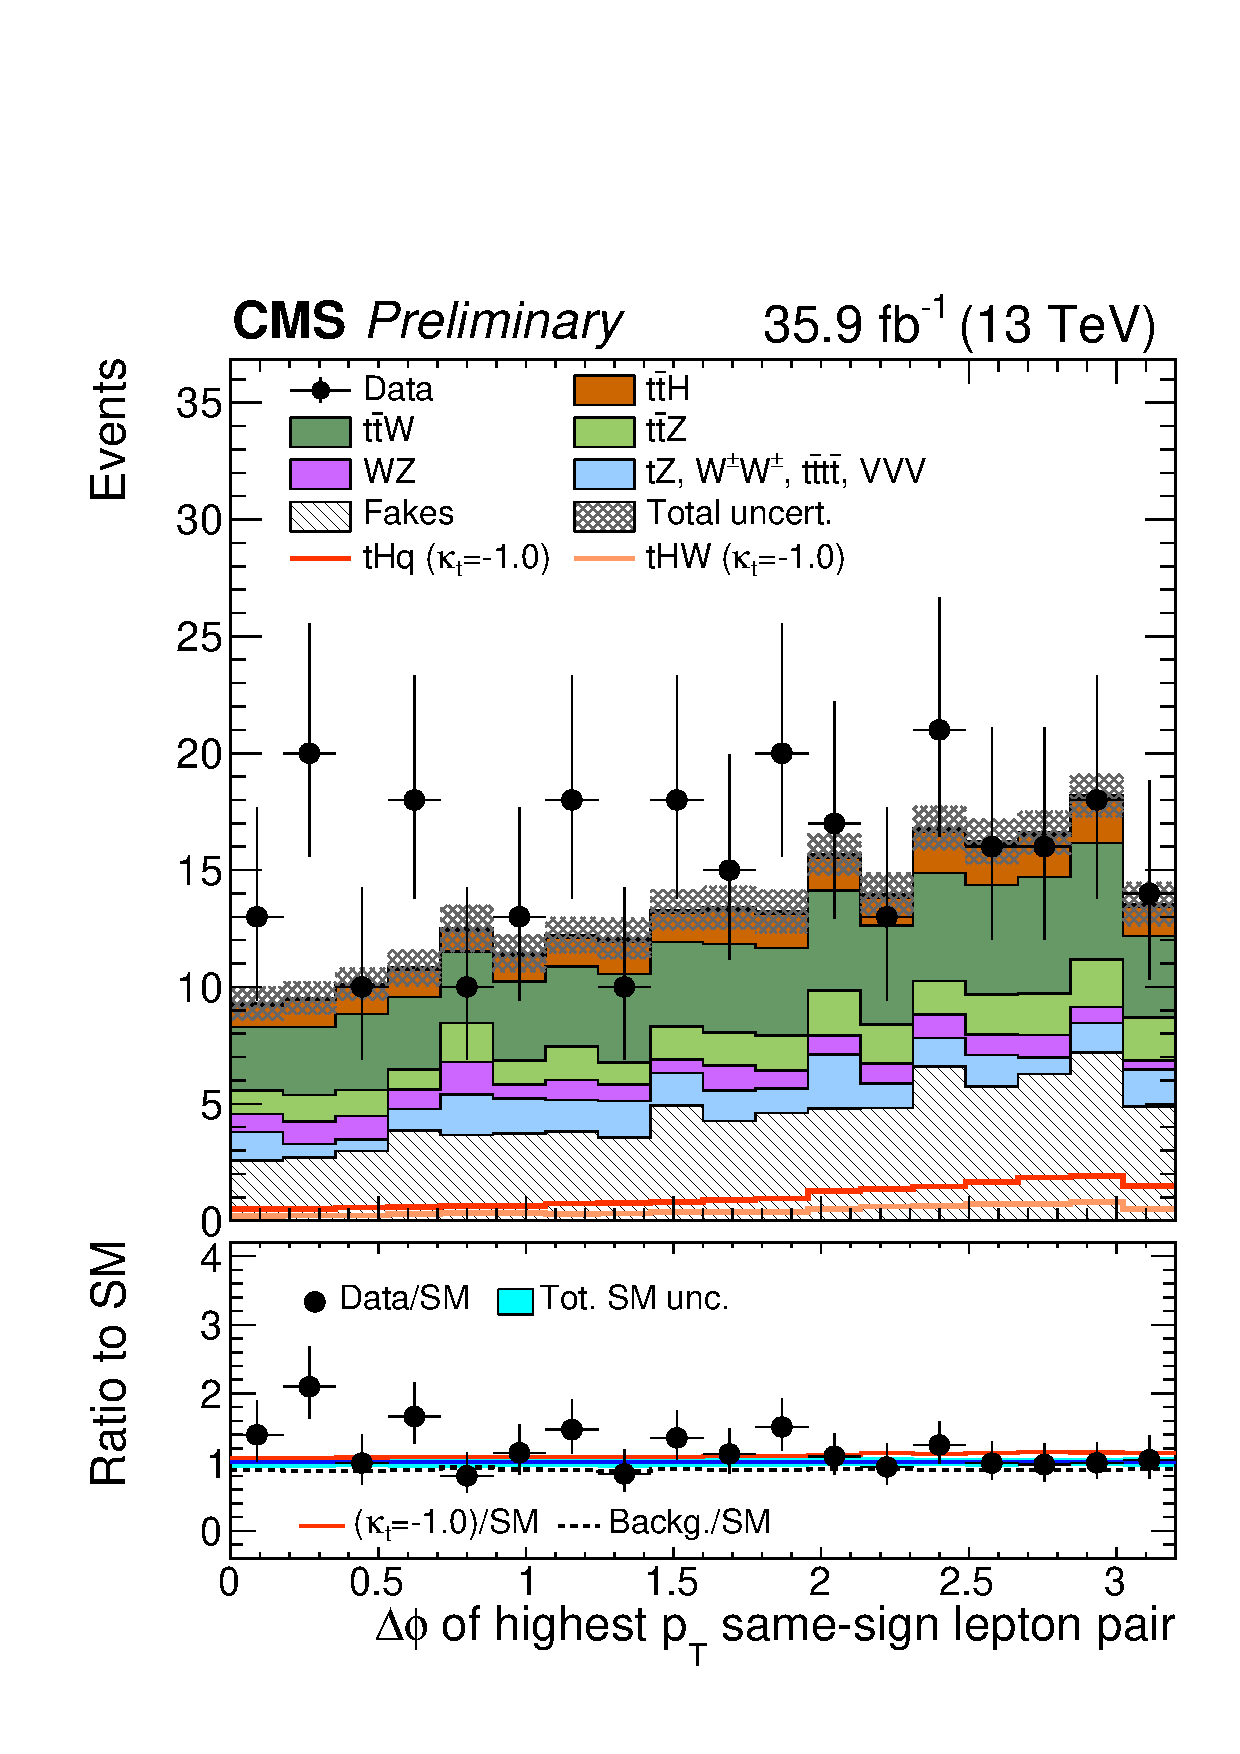
\includegraphics[width=0.32\linewidth]{Figures/polished/dPhiHighestPtSSPair_mm.pdf}
    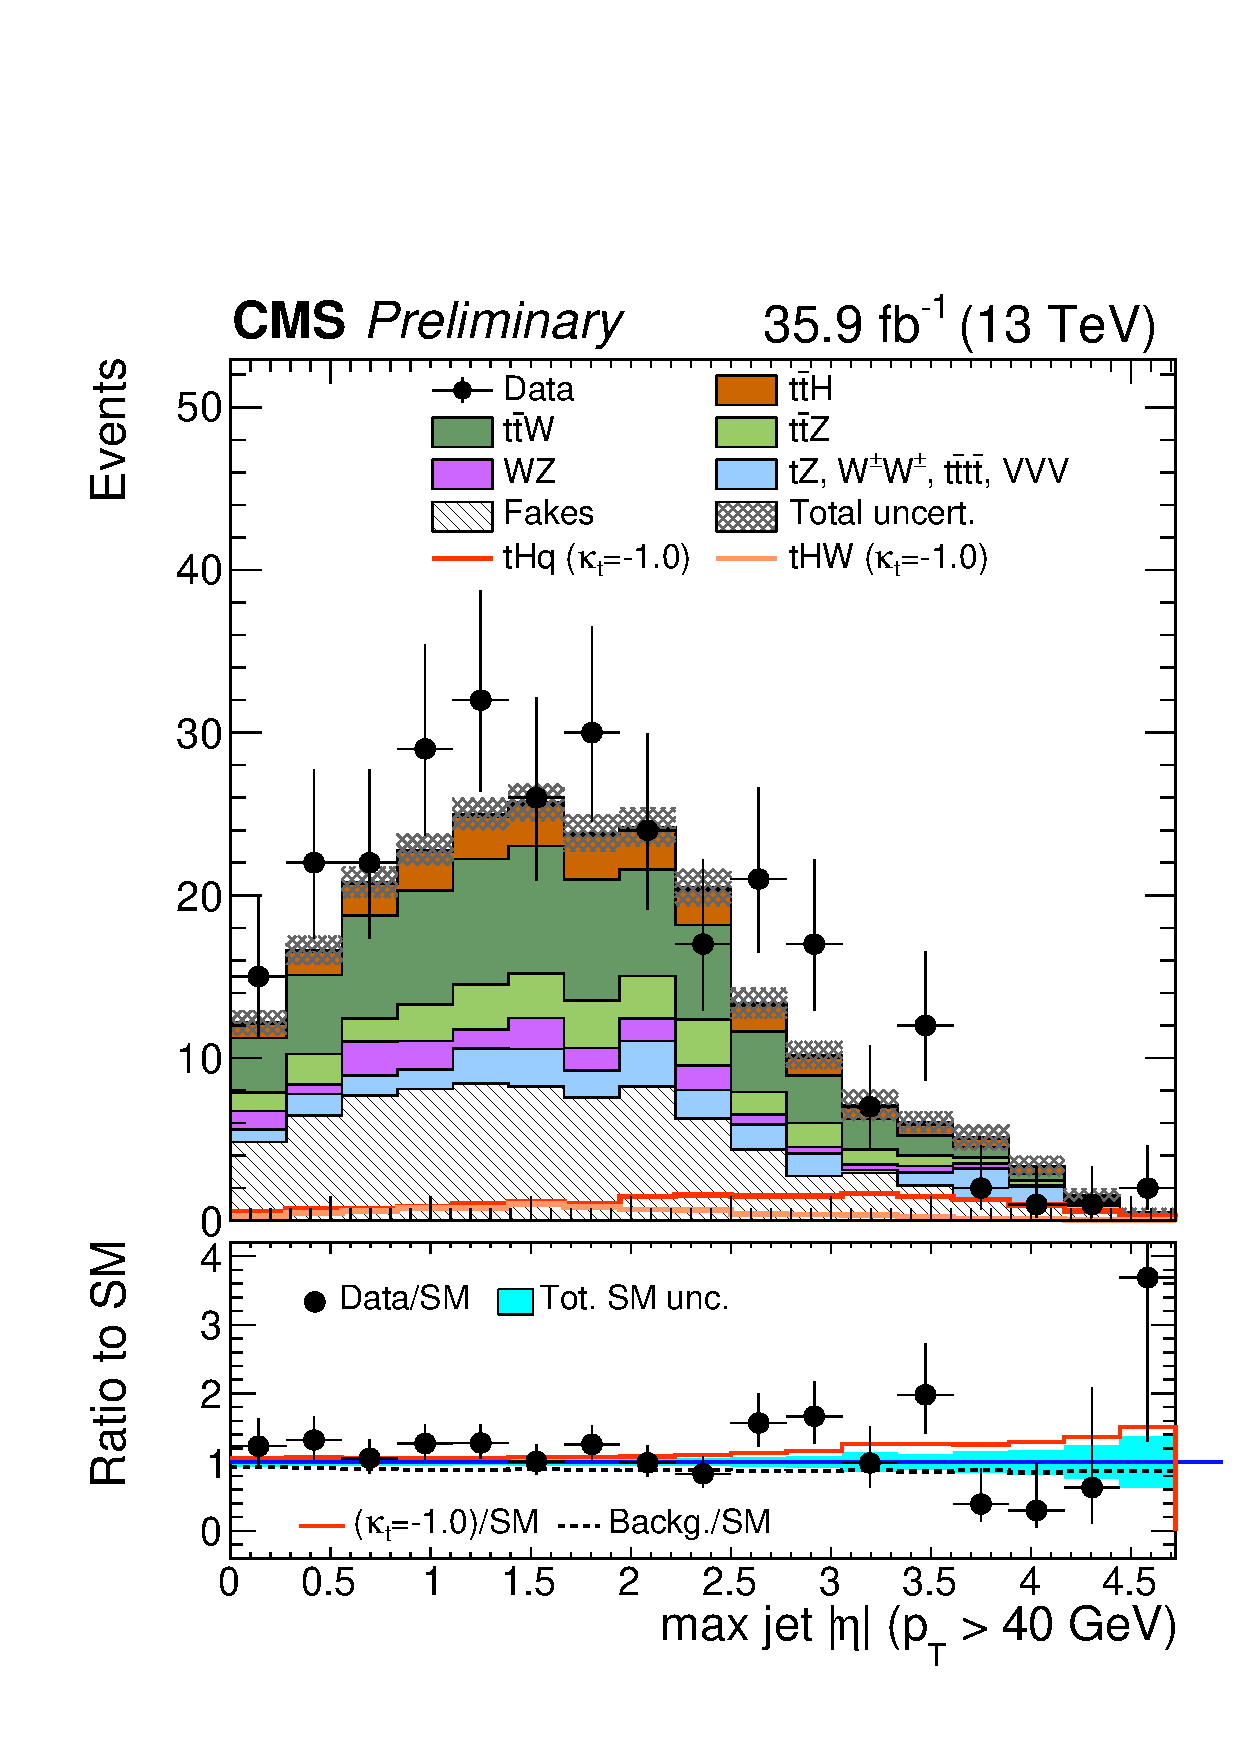
\includegraphics[width=0.32\linewidth]{Figures/polished/maxEtaJet25_40_mm.pdf}
    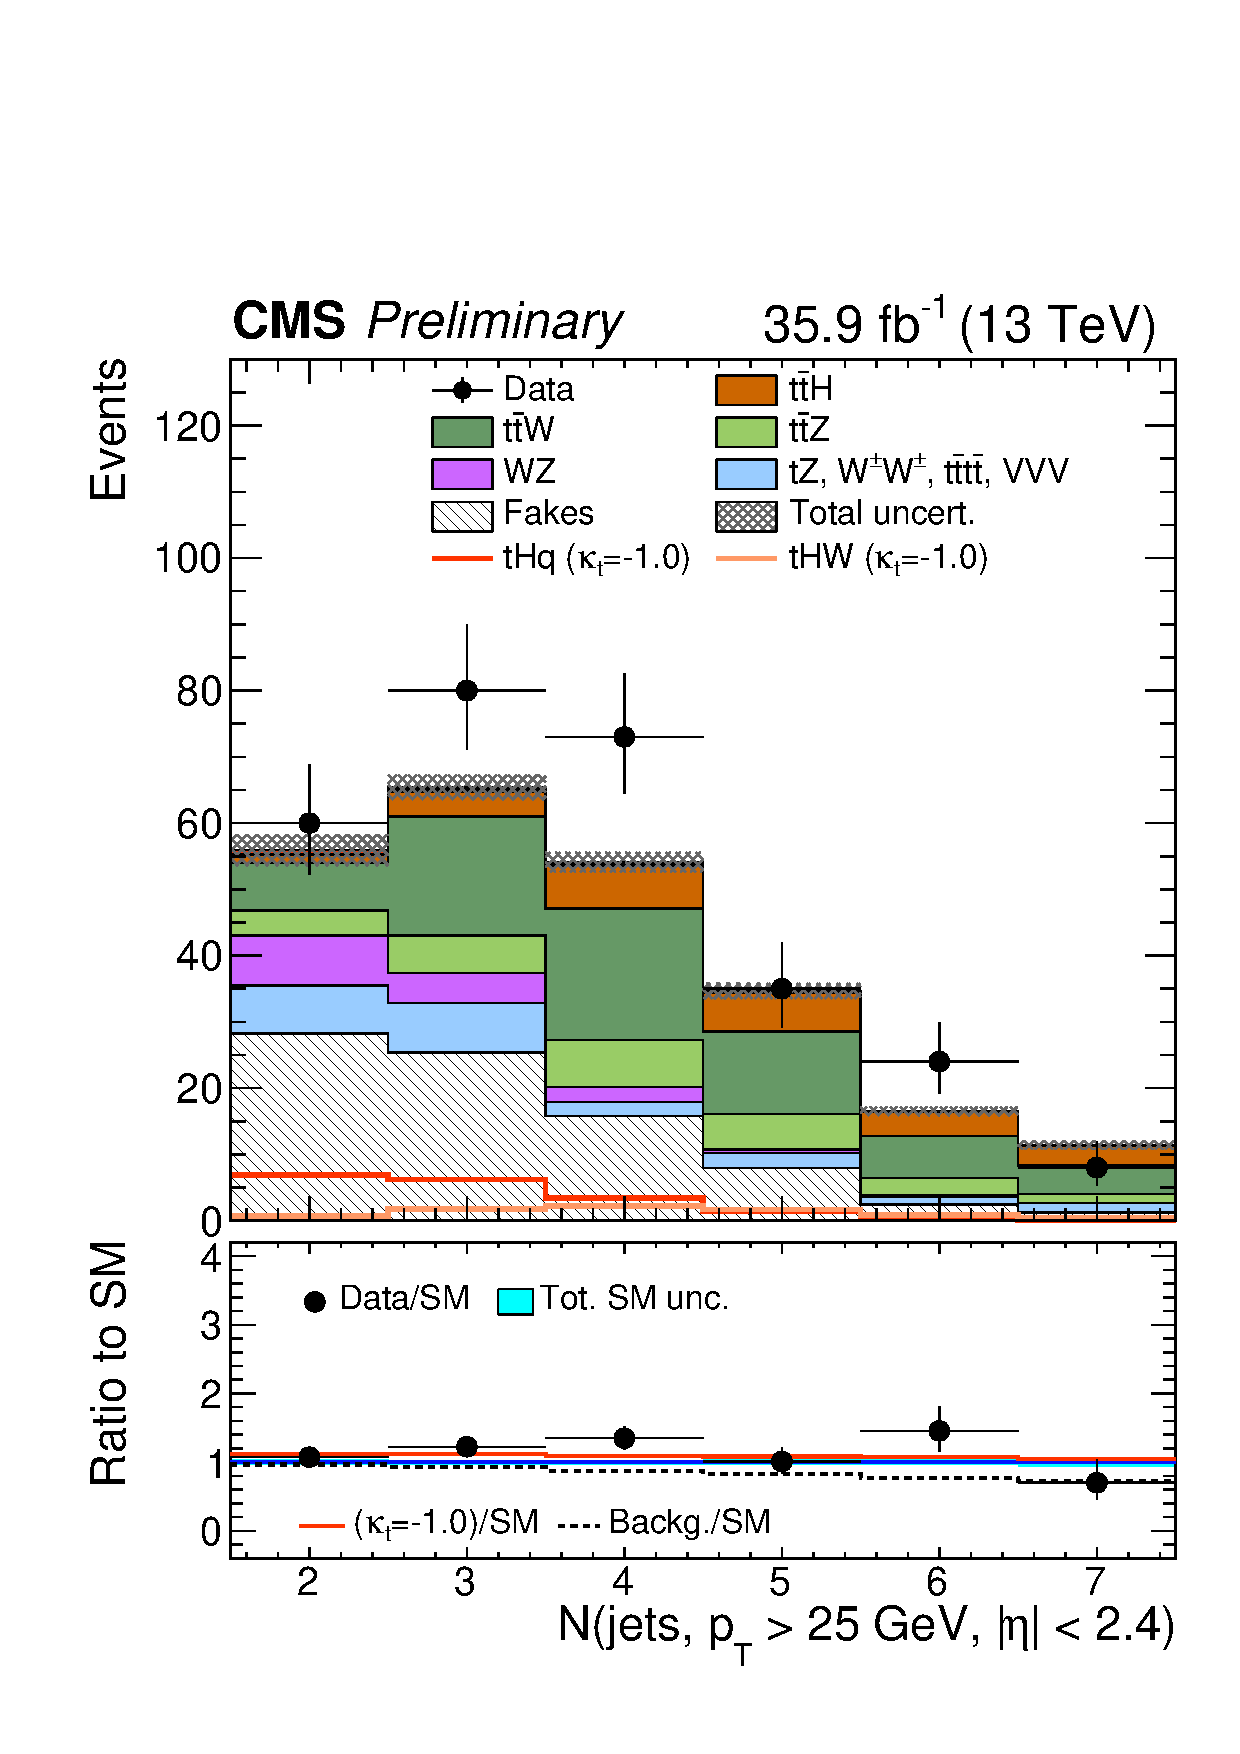
\includegraphics[width=0.32\linewidth]{Figures/polished/nJet25_mm.pdf} \\
  \caption{Distributions of discriminating variables for the event pre-selection for the same-sign \mumu\ channel, normalized to 35.9\fbinv, before fitting the signal discriminant to the observed data.
  Uncertainties are statistical and unconstrained (pre-fit) normalization systematics.
  The shape of the two \tH\ signals for $\Ct=-1.0$ is shown, normalized to their respective cross sections for $\Ct=-1.0, \CV=1.0$.\label{fig:2lss_inputs_mm}}
\end{figure}

\begin{figure}[!htb]
  \centering
    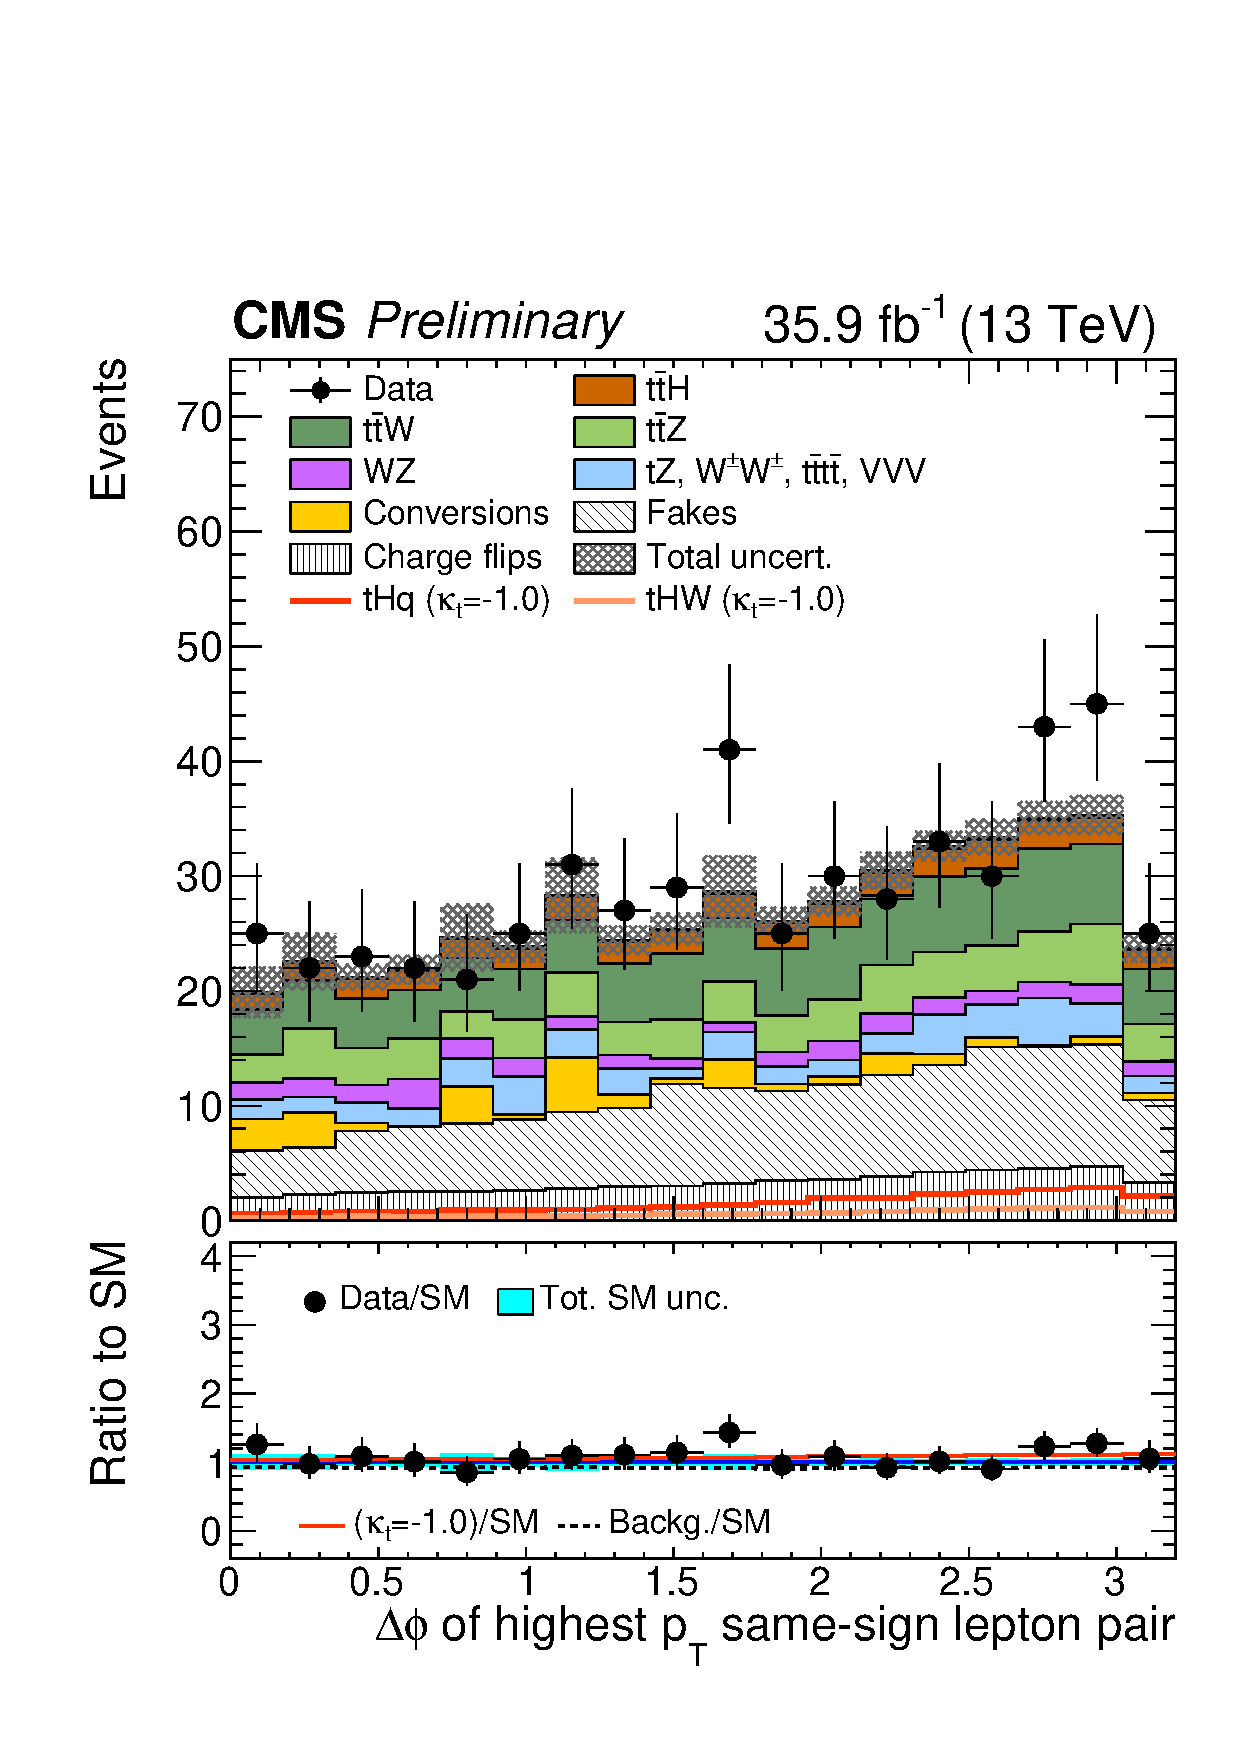
\includegraphics[width=0.32\linewidth]{Figures/polished/dPhiHighestPtSSPair_em.pdf}
    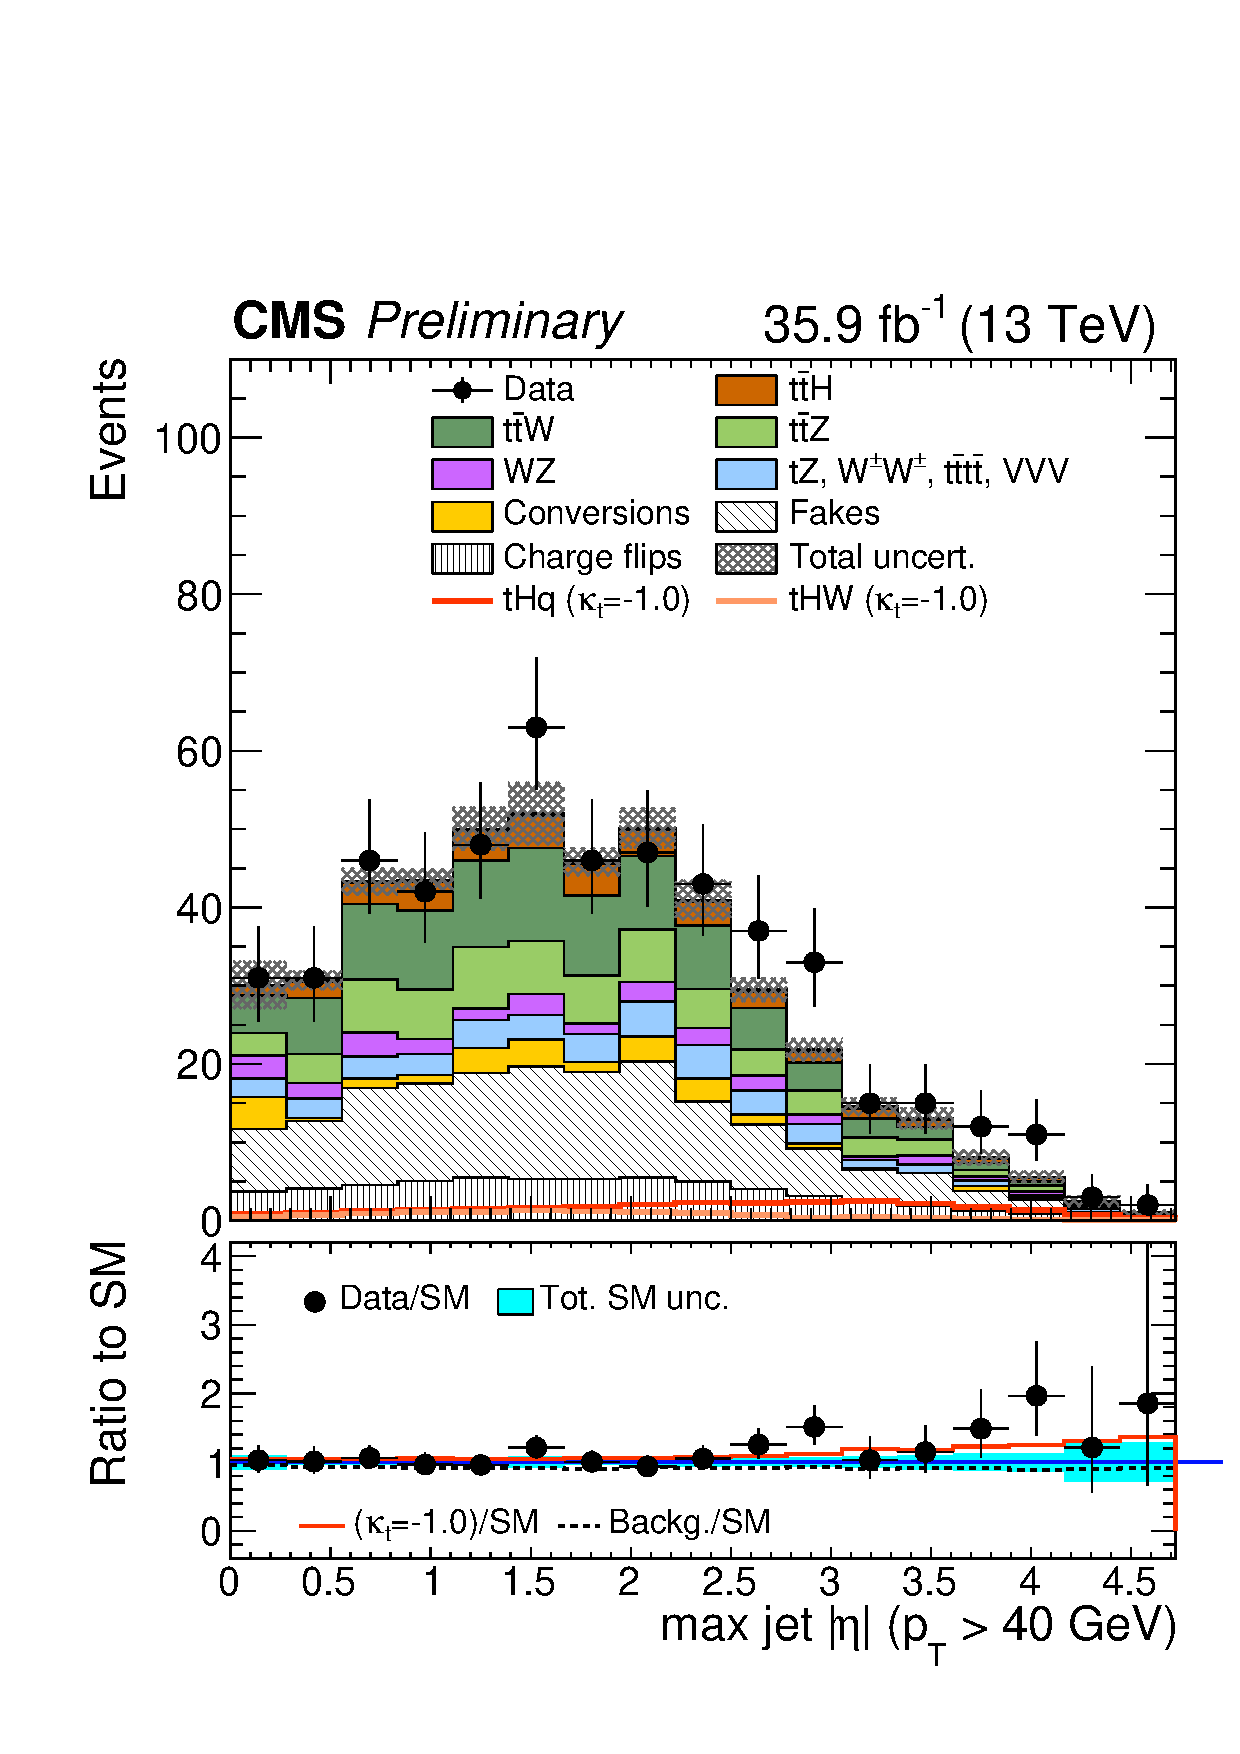
\includegraphics[width=0.32\linewidth]{Figures/polished/maxEtaJet25_40_em.pdf}
    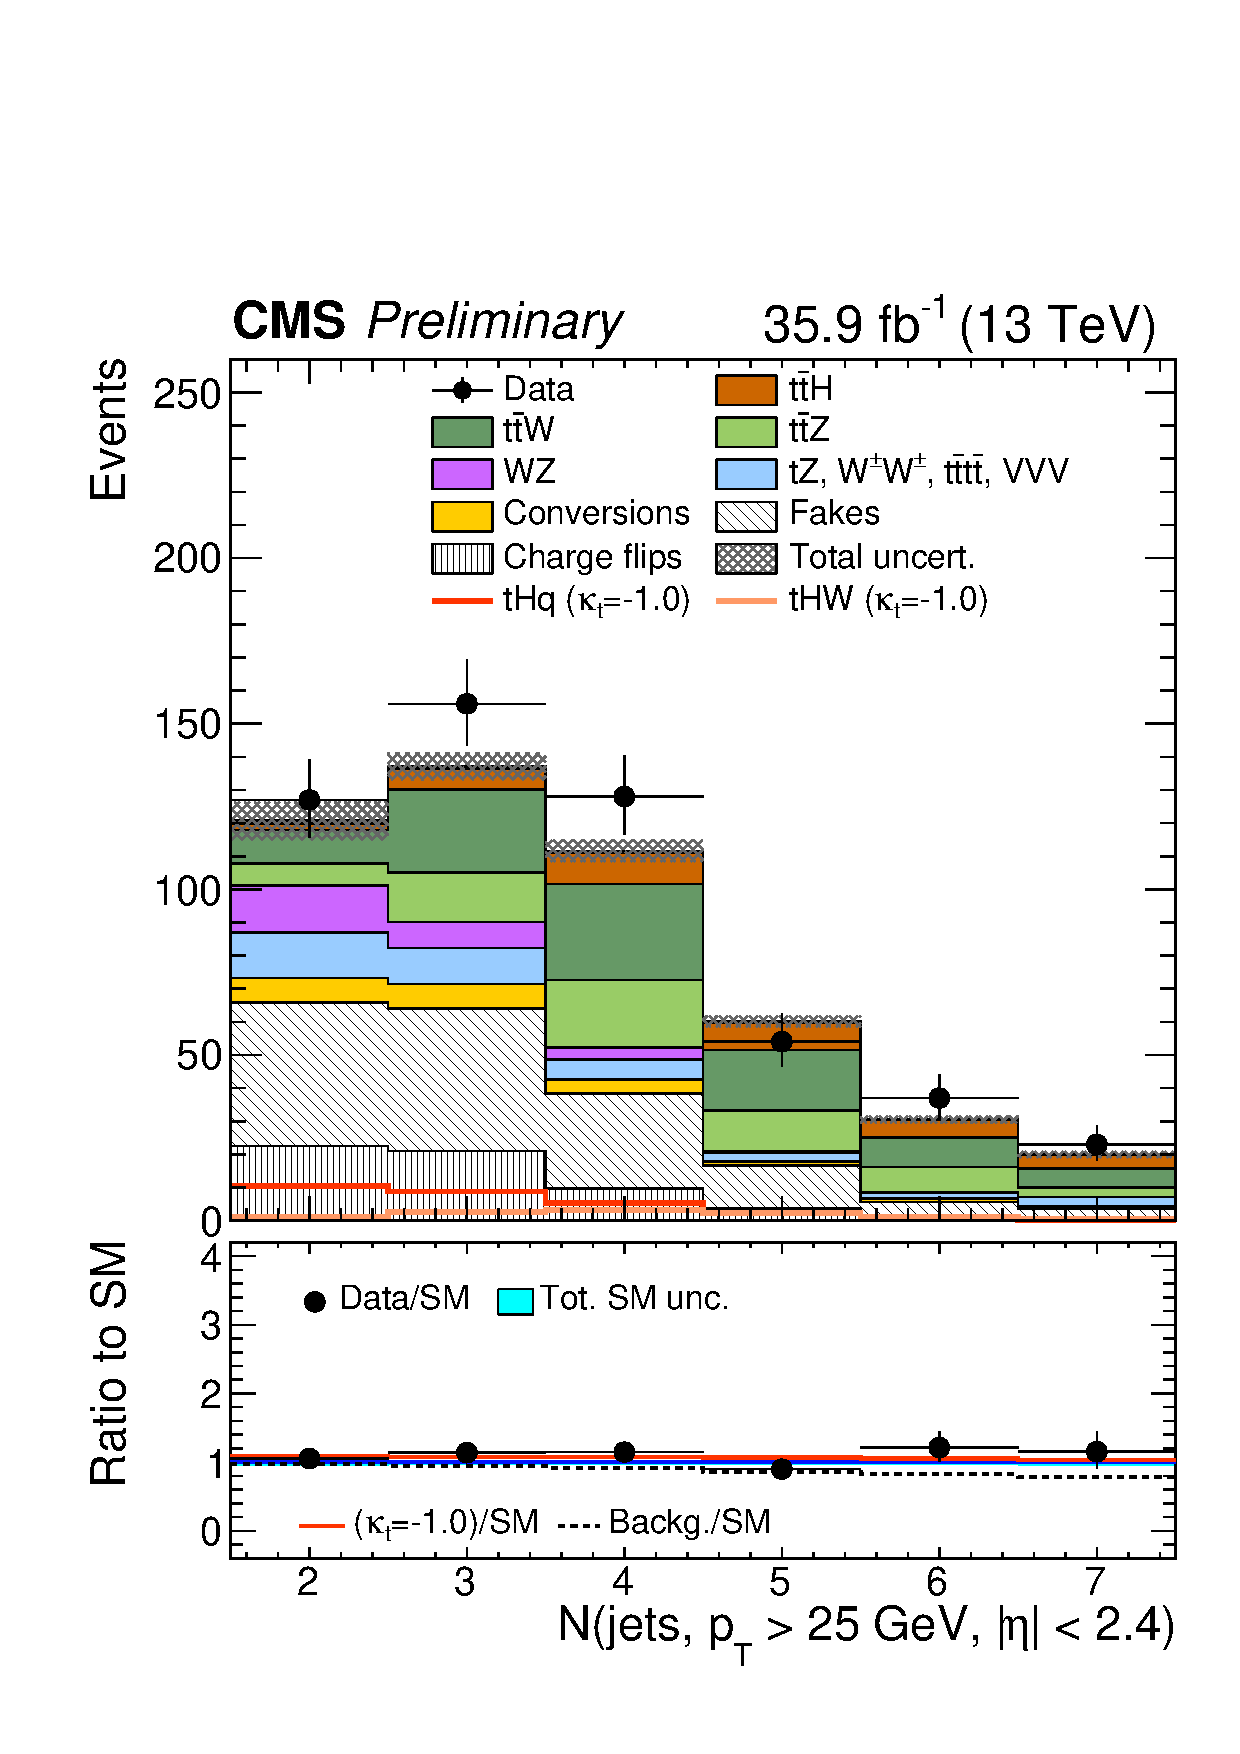
\includegraphics[width=0.32\linewidth]{Figures/polished/nJet25_em.pdf} \\
  \caption{Distributions of discriminating variables for the event
    pre-selection for the same-sign \emu\ channel, normalized to 35.9\fbinv, before fitting the signal discriminant to the observed data. Uncertainties are statistical and unconstrained (pre-fit) normalization systematics.
    The shape of the two \tH\ signals for $\Ct=-1.0$ is shown, normalized to their respective cross sections for $\Ct=-1.0, \CV=1.0$.\label{fig:2lss_inputs_em}}
\end{figure}

\begin{figure}[!htb]
  \centering
    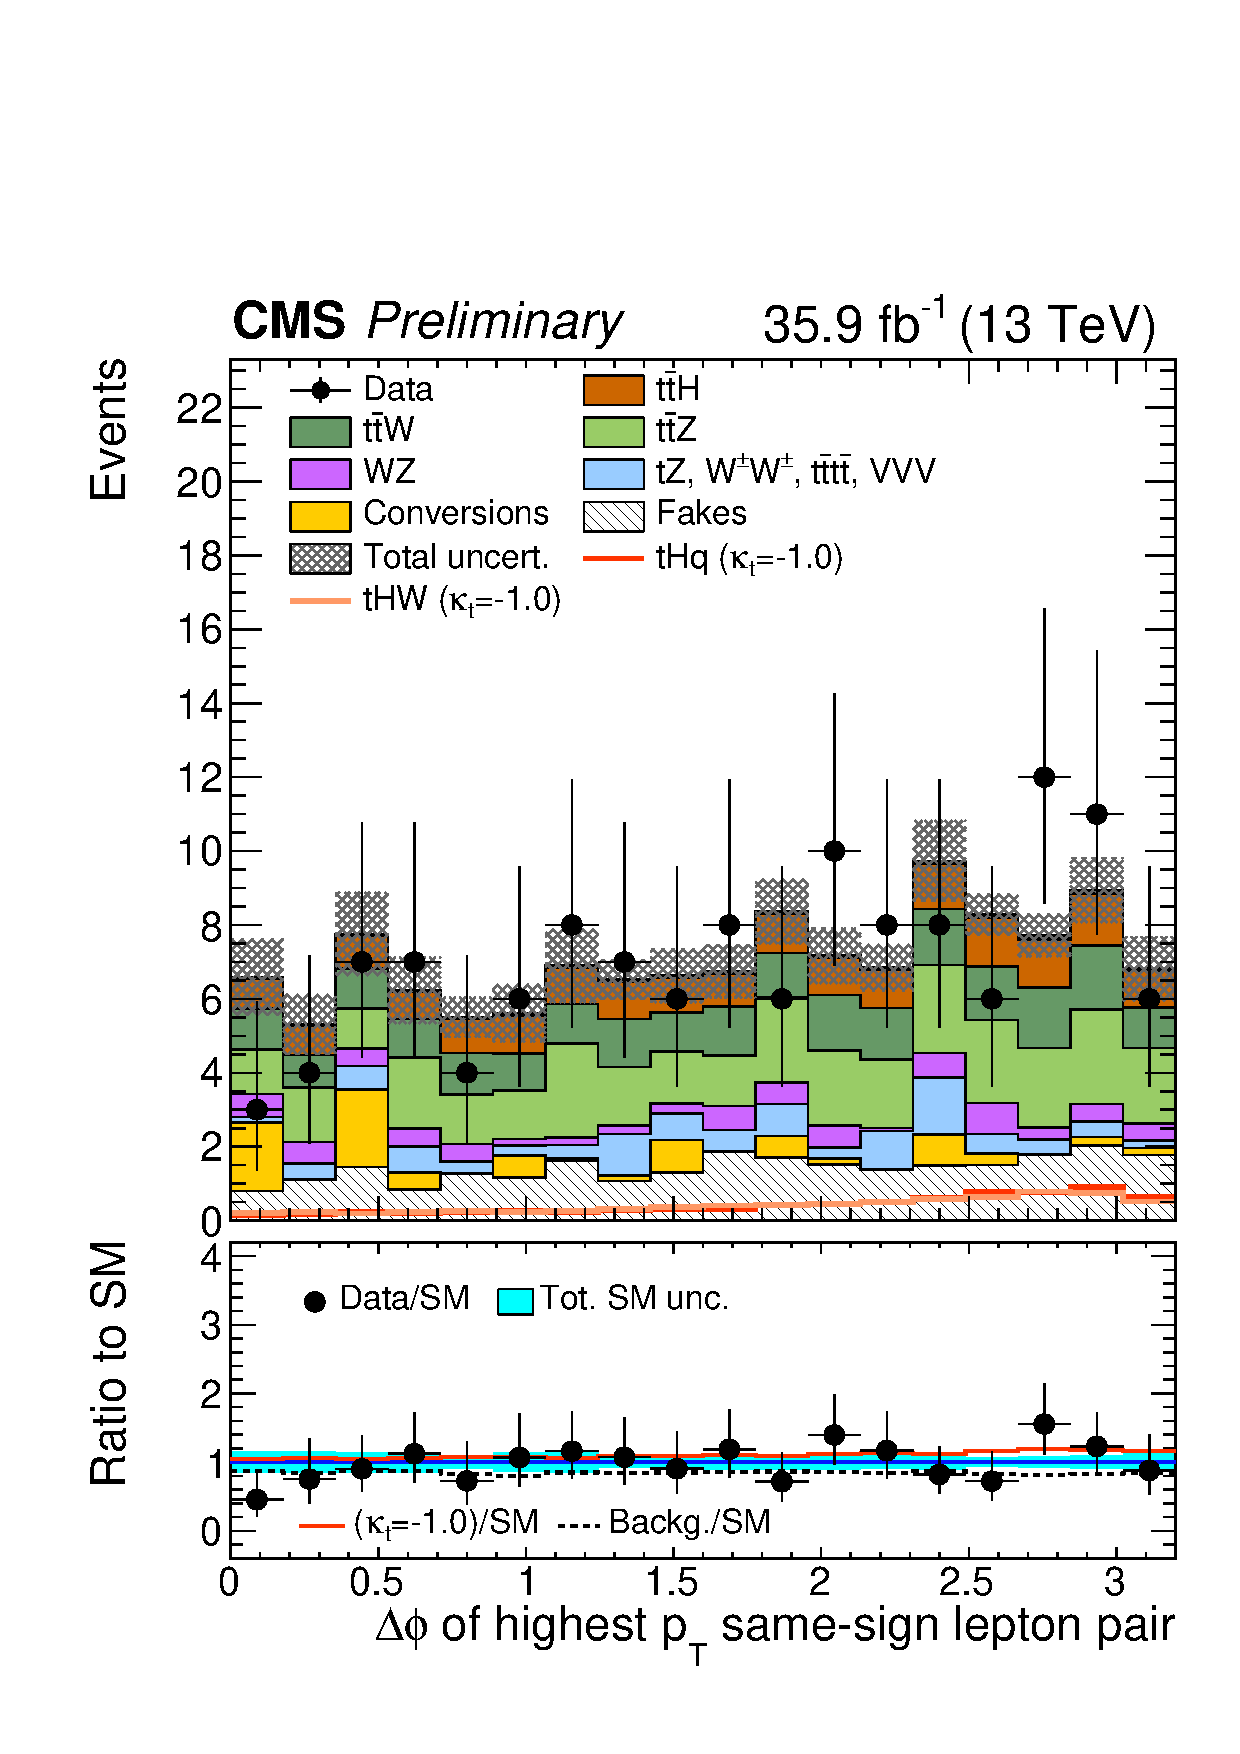
\includegraphics[width=0.32\linewidth]{Figures/polished/dPhiHighestPtSSPair_3l.pdf}
    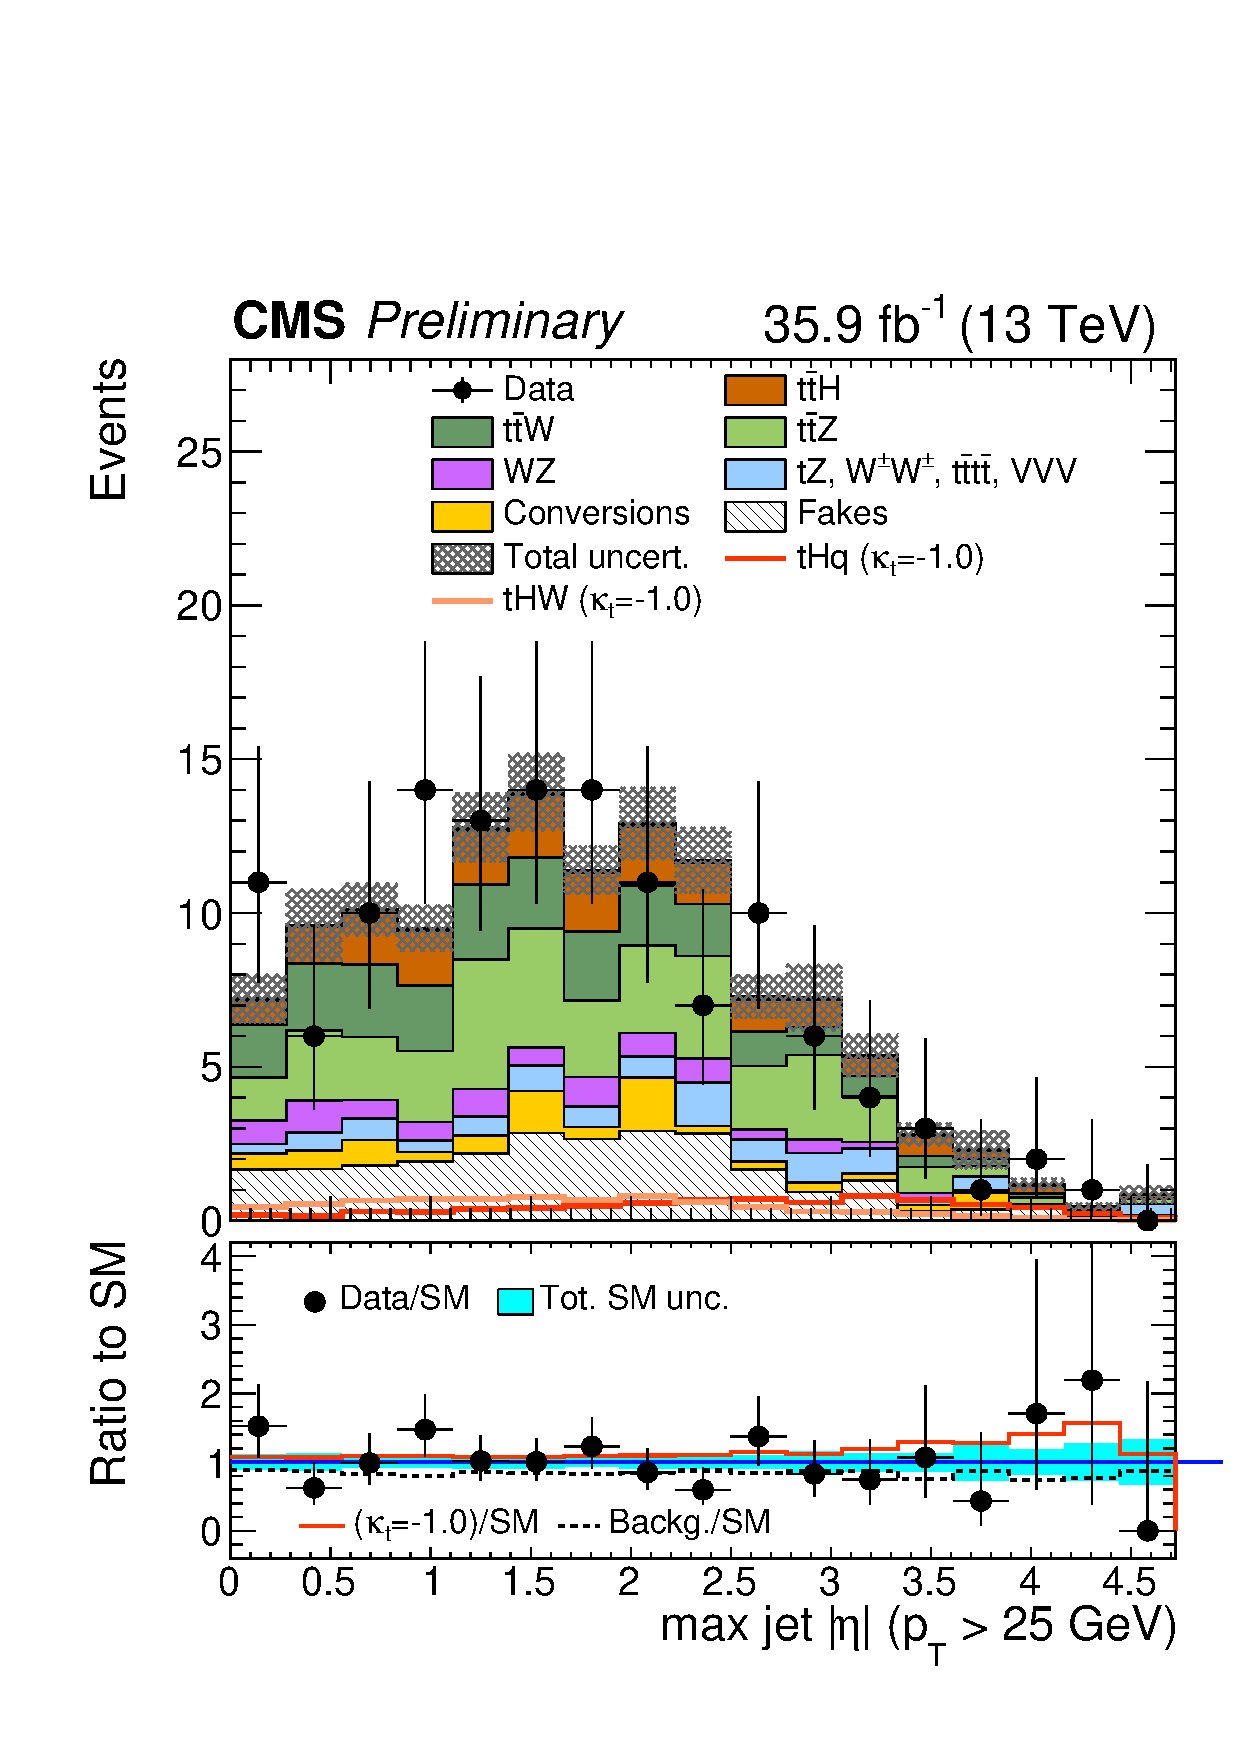
\includegraphics[width=0.32\linewidth]{Figures/polished/maxEtaJet25_40_3l.pdf}
    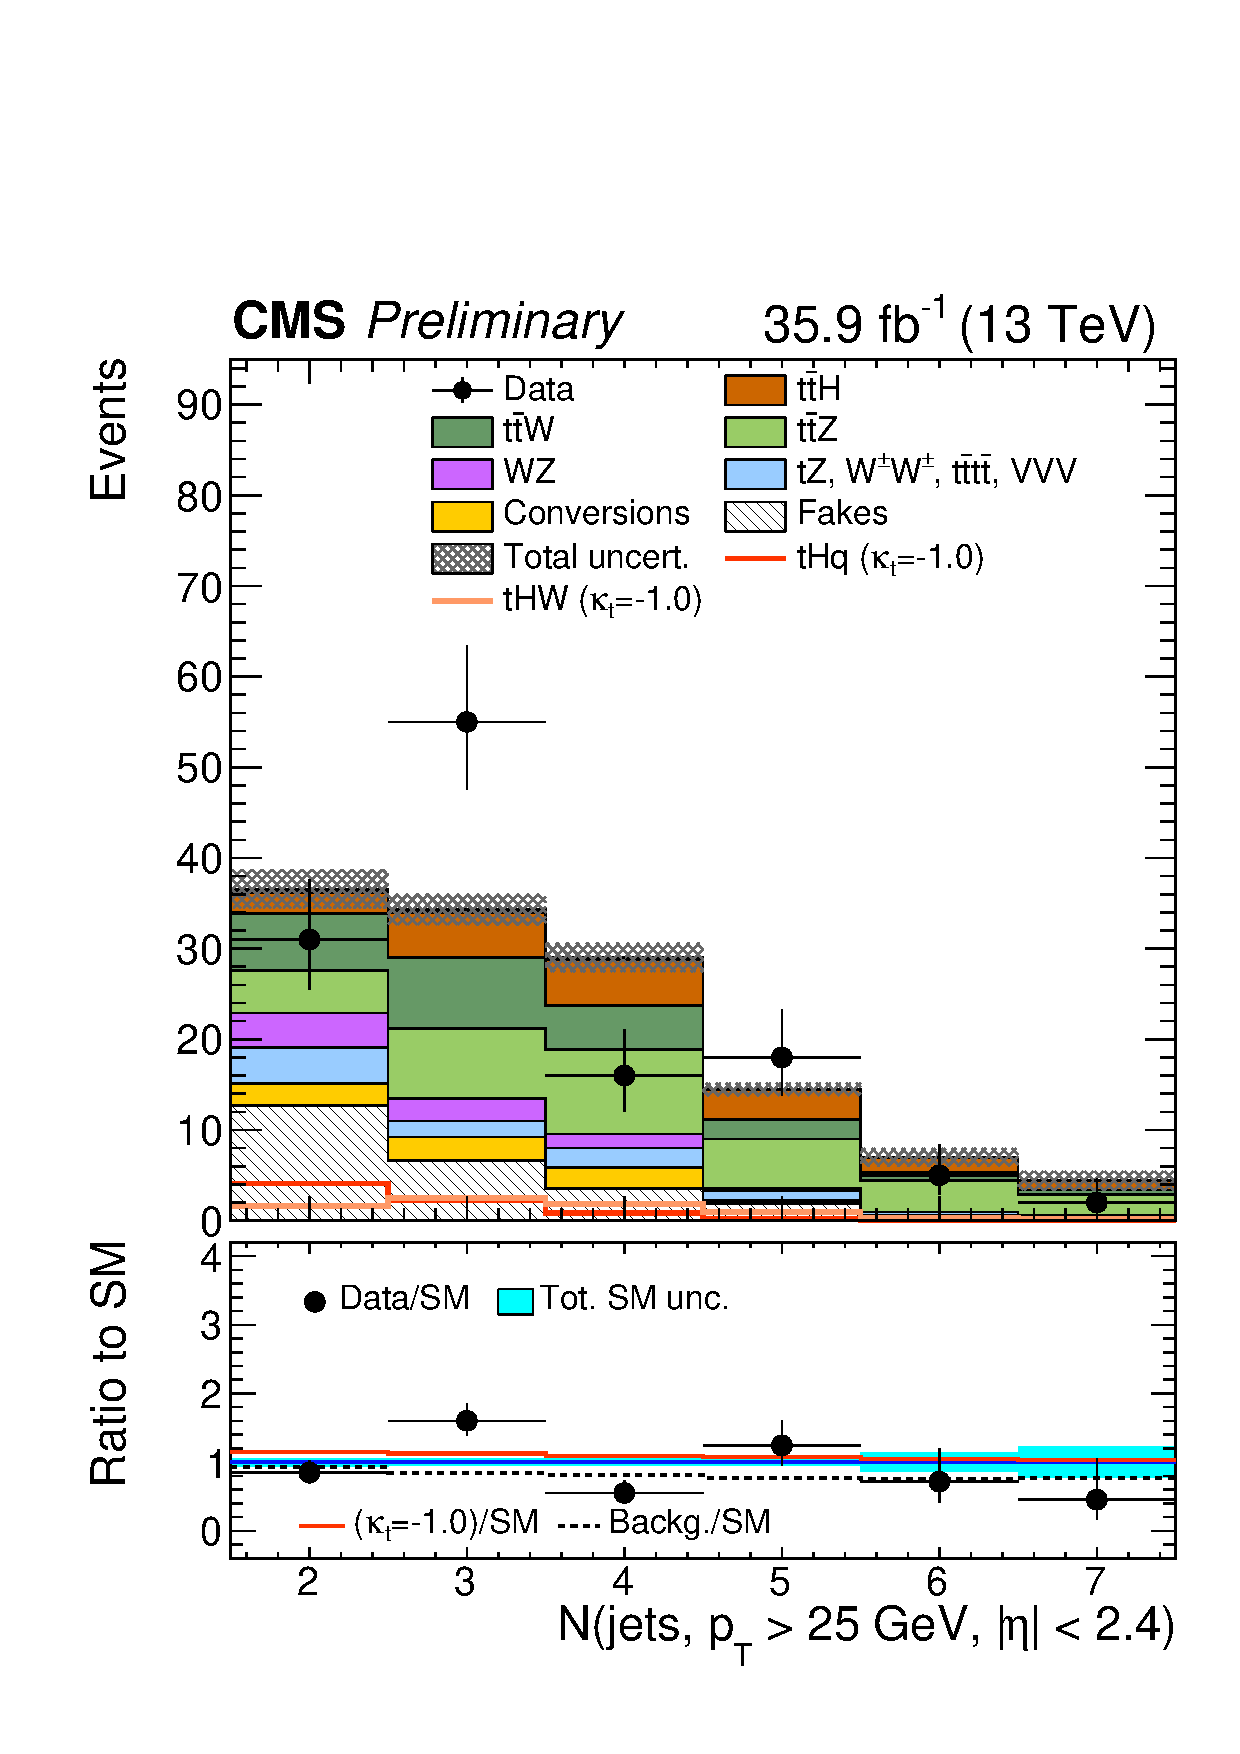
\includegraphics[width=0.32\linewidth]{Figures/polished/nJet25_3l.pdf} \\
  \caption{Distributions of discriminating variables for the event pre-selection for the three lepton channel, normalized to 35.9~\fbinv, before fitting the signal discriminant to the observed data.
  Uncertainties are statistical and unconstrained (pre-fit) normalization systematics.
  The shape of the two \tH\ signals for $\Ct=-1.0$ is shown, normalized to their respective cross sections for $\Ct=-1.0, \CV=1.0$.\label{fig:dist_likelihoodselection_PDFs_3l}}
\end{figure}


% MC generators, theory systematics, irreducible backgrounds
%% These input names don't make much sense...
\section{Modeling of signal and background processes}\label{sec:experiment}
The \tHq\ and \tHW\ signal events are generated using \textsc{MG5\_}a\textsc{MC@NLO} (version 5.222)~\cite{amcatnlo} at leading-order precision, using the \textsc{MLM} merging scheme~\cite{Alwall:2007fs} and the \textsc{NNPDF3.0} PDF set~\cite{Ball:2014uwa}, and are normalized to next-to-leading order cross sections.
The \tHq\ events are generated with the four-flavor scheme while the \tHW\ process uses the five-flavor scheme to eliminate leading-order interference with the \ttH\ process~\cite{Demartin:2016axk}.
Event weights are produced in the generation of both samples to allow a reshaping of observables for 51 different coupling configurations: $17$ values of \Ct\ between $-3.0$ and $+3.0$ for three values of \CV: $+0.5$, $+1.0$, and $+1.5$, corresponding to 33 unique values of $\Ct/\CV$, ranging from $-6.0$ to $6.0$, and therefore 33 distinct kinematic configurations.

\textsc{MG5\_}a\textsc{MC@NLO} in NLO mode is used for the \ttH\ process and the main backgrounds: \ttW, \ttZ, \ttbar+jets, and $\ttbar\gamma$+jets, using parton-shower merging at NLO~\cite{Frederix:2012ps}.
Other minor backgrounds are simulated with different generators, such as \textsc{POWHEG}~\cite{Nason:2004rx,Frixione:2007vw,Alioli:2010xd,Re:2010bp,Alioli:2009je,Melia:2011tj} and \MADGRAPH\ at leading order (LO) QCD accuracy.
All generated events are interfaced to \textsc{Pythia8} (v8.205)~\cite{PYTHIA8} for the parton shower and hadronization steps.
Pileup interactions are simulated to reflect the observed multiplicity in data.
The simulated events are weighted according to the actual pileup in data, estimated from the measured bunch-to-bunch instantaneous luminosity and the total inelastic cross section, 69.2 mb.
All events are finally passed through a full simulation of the CMS detector based on \GEANTfour~\cite{GEANT}, and reconstructed using the same algorithms as used for the data.

Furthermore, the trigger selection is simulated and applied for generated signal events.
Residual differences in the trigger efficiency between data and MC are studied and corrected for, using the measured trigger efficiencies of the data.

\subsection{Signal modeling}\label{sec:syst}
Systematic uncertainties on the signal selection efficiency arise from correction factors applied to the simulated events to better match the measured detector performance and also from theoretical uncertainties in the modeling of the signal process.

Scale factors applied to correct for data/MC differences in the trigger efficiency, lepton reconstruction and identification performance, and lepton selection efficiency carry a combined uncertainty of about 5\% per lepton.
The impact of the uncertainty in the signal selection efficiency from jet energy corrections is evaluated by varying the correction factors within their uncertainty and propagating the effect to the final result by recalculating all kinematic quantities.
Effects on the overall normalization of event yields and on the shape of kinematic properties are both taken into account.
Jet energy resolution effects have negligible impact on this analysis.
Correction factors for data/MC differences in the \cPqb-tagging performance are applied depending on the \pt\ and $\eta$, and on the flavor of the jet, and their effect on the signal efficiency is evaluated by varying the factors within their measured uncertainty and recalculating the overall event scale factors.

The uncertainties from unknown higher orders of \tHq\ and \tHW\ production are estimated from a change in the $Q^2$ scale of double and half the initial value, evaluated for each point of \Ct\ and \CV.
The \ttH\ signal component has an uncertainty of about $+5.8/\!-9.2\%$ from $Q^2$ scale variations and a further $3.6\%$ from the knowledge of PDFs and $\alpha_S$~\cite{deFlorian:2016spz}.

% This varies both the overall rate and the shape of kinematic distributions for the simulated signal events.
Uncertainties related to the choice of PDF set and its scale are estimated to be about $3.7\%$ for \tHq\ and about $4.0\%$ for \tHW. %% FIXME Citation

\subsection{\ttV, \WZ, and \ZZ\ backgrounds}
%\subsection{\ttbar+vector boson backgrounds and \ttH\ signal}
Backgrounds from associated production of \ttbar\ pairs and electroweak bosons (\ttW\ and \ttZ) are estimated directly from simulated events, which are corrected for data/MC differences and inefficiencies in the same way as signal events.
Their production cross sections are calculated at next-to-leading order of QCD and EWK, with theoretical uncertainties from unknown higher orders of $12\%$ for \ttW\ and $10\%$ for \ttZ.
Further uncertainties arise from the knowledge of PDFs and $\alpha_S$ of about $4\%$ each for \ttW\ and \ttZ.

%\subsection{\WZ\ and \ZZ\ backgrounds}
Diboson production with leptonic \Z\ decays and additional jet radiation in the final state can lead to signatures very similar to that of the signal.
Due to the larger cross section, the main contribution arises from \WZ\ production.
Inclusive production cross sections for both \WZ\ and \ZZ\ have been measured at the LHC and agree well with the NLO calculations.%% FIXME Reference
 However, the good agreement of the cross section measurements in the inclusive phase space does not necessarily hold in the signal region of this analysis, which requires the presence of hadronic jets, including \cPqb\ jets.
Therefore, a dedicated control region dominated by \WZ\ production is used to constrain the overall normalization of this process.
It is defined by the presence of at least three leptons, of which one opposite-sign pair must be compatible with a \Z\ boson decay.
Furthermore, at least two jets are required, with a veto on jets that pass the loose \cPqb\ tag selection to ensure exclusivity with the signal selection.
A scale factor is then extracted from the predicted distribution of \WZ\ events in the control region, and the observed data, keeping other processes fixed.
Finally, this factor is used to scale the diboson prediction in the signal selection.

The majority of diboson events passing the signal selection contain jets from light quarks and gluons that are incorrectly tagged as \cPqb\ jets, making this estimate mainly sensitive to the experimental uncertainty in the mis-tag rate rather than the theoretical uncertainty in the jet flavor composition.
The overall uncertainty assigned to the diboson prediction is estimated from the statistical uncertainty due to the limited sample size in the control region (30\%), the residual background in the control region (20\%), the uncertainties on the \cPqb-tagging rate (10--40\%), and from the knowledge of PDFs and the theoretical uncertainties of the extrapolation (up to 10\%). %% FIXME: Check these numbers


\subsection{Non-prompt and charge mis-identified leptons}\label{sec:fakes}
The main contribution to the overall event yield in the signal selection, and one that can be reduced up to a certain point by tighter lepton selections, comes from processes with comparatively large cross sections in which one of the leptons is produced inside a jet (\ie\ it is non-prompt).
These are mostly real leptons from \cPqb\ hadron decays but also contain hadronic jets misidentified as leptons.
The yield of such events is estimated from a loose-to-tight extrapolation, in which a looser lepton selection is defined and the rate at which such leptons enter the tighter selection is measured in a control region and then used to extrapolate from a sideband with loose leptons to the signal selection with tight leptons.

The probability of a non-prompt lepton candidate passing a given loose selection to also pass the tight signal requirement is measured in a sample dominated by non-prompt leptons, as a function of \pt\ and $|\eta|$ and separately for muons and electrons.
The definitions of loose and tight leptons are given in Sec.~\ref{sec:objects}.
Two event samples are defined for the measurement of tight-to-loose ratios: one dominated by QCD multijet events, collected using single lepton triggers at relatively high \pt\ thresholds; and one dominated by $\Z+\mathrm{jets}$ events, where the two high \pt\ leptons from the \Z\ decay can be used to trigger the events without biasing the \pt\ spectrum of a third lepton at low transverse momentum.
The QCD-dominated sample is then used to extract ratios for lepton candidates with \pt\ above 30\GeV, whereas the ratios for low \pt\ leptons are determined in the $\Z+\mathrm{jets}$ sample.
For both regions, contributions from prompt leptons, mainly from \PW\ and $\Z+\mathrm{jets}$ or from \WZ\ and \ZZ\ events, respectively, are first suppressed by vetoing additional leptons in the selection, and the residual contamination is then subtracted using the transverse mass as a discriminating variable.  %Lepton-MET transverse mass?  Presumably, but would be good to say.

A sideband control region is then defined by relaxing the lepton selection criteria to ``loose'' (see Sec.~\ref{sec:objects}), while keeping all other selections equivalent to the full signal selection.
By weighting events in this expanded selection with a factor dependent on the measured tight-to-loose ratios, a fully data-driven estimation for the contribution of non-prompt leptons to the signal selection can be obtained.
In events where just one of the two leptons fails the tight criteria, the applied event weight is $f/(1-f)$ (where $f$ is the tight-to-loose ratio measured as described above), while events where both leptons fail the tight criteria are weighted by $-f_1f_2/[(1-f_1)(1-f_2)]$.
The resulting prediction of the event yield in the signal selection carries an uncertainty of 30--50\%, arising from the statistical uncertainty in the measurement of the tight-to-loose ratios, and from a systematic uncertainty derived by comparing alternative methods of subtracting prompt lepton backgrounds and from testing the closure of the method in simulated background events.

Similarly, background from events where the charge of one of the leptons is wrongly assigned---relevant only in the same-sign dilepton channels---are determined by measuring the charge mis-assignment probability in a sample of same-sign dilepton event compatible with a \Z\ boson decay and weighting events with opposite-sign leptons in the signal selection.
The charge mis-assignment probability is found to be negligible for this analysis for muons, whereas for electrons it ranges from about 0.02\% in the barrel section ($|\eta| < 1.48$) up to about 0.4\% in the detector endcaps ($ 1.48 < |\eta| < 2.5$).
It is measured separately in these two regions, and additionally as a function of the electron \pt.
A systematic uncertainty of 30\% is assigned to the prediction from the statistical uncertainty of the probability measurement and from testing the performance of the method on simulated events.
 % Fake rate and charge flip backgrounds

% Limits and signal strengths
\section{Results}\label{sec:results}
After applying the event pre-selection on the dataset, $280$ events are observed in the same-sign \mumu\ channel, $525$ in the same-sign \emu\ channel, and $149$ events in the trilepton channel (\threel).
The events are then sorted into ten categories depending on the output of the two BDT classifiers according to an optimized binning strategy, resulting in a one-dimensional histogram with ten bins.
The expected signal and background shapes for this distribution are then fit to the observed data in a maximum likelihood fit, simultaneously for all three channels and separately for the signal shapes for each of the 33 $\Ct/\CV$ coupling configuration points.

In each point, the \tH\ and \ttH\ production cross sections and the Higgs decay branching ratios are modified with the Higgs-top (\Ct) and Higgs-vector boson (\CV) coupling strength.
The Higgs-tau coupling strength modifier ($\kappa_\tau$) is assumed to be equal to \Ct.
% This includes modified branching ratios of $\PH\to\gamma\gamma$, $\PH\to\Z\gamma$, and $\PH\to\Pg\Pg$ with varying \Ct, and an accordingly adjusted overall Higgs decay width. % FIXME?
All other parameters are assumed to be at the values predicted by the standard model.
This implies that the combined signal shape is uniquely defined by the ratio of $\Ct/\CV$.
In the fit, the \tH\ and \ttH\ signal are then floated with a common signal strength modifier (defined as the ratio to the expected cross section) to produce a 95\% confidence level (C.L.) upper limit on the observed $\tH+\ttH$ cross section times the combined branching ratio of $\PH\to\W\W^*+\tautau+\Z\Z^*$.

The pre-fit BDT output distributions are shown in Fig.~\ref{fig:postfitshapes}, whereas Fig.~\ref{fig:finalbins} shows the post-fit categorized BDT output distributions obtained in the maximum likelihood fit to extract the limits.

\begin{figure}[!htb]
  \begin{center}
    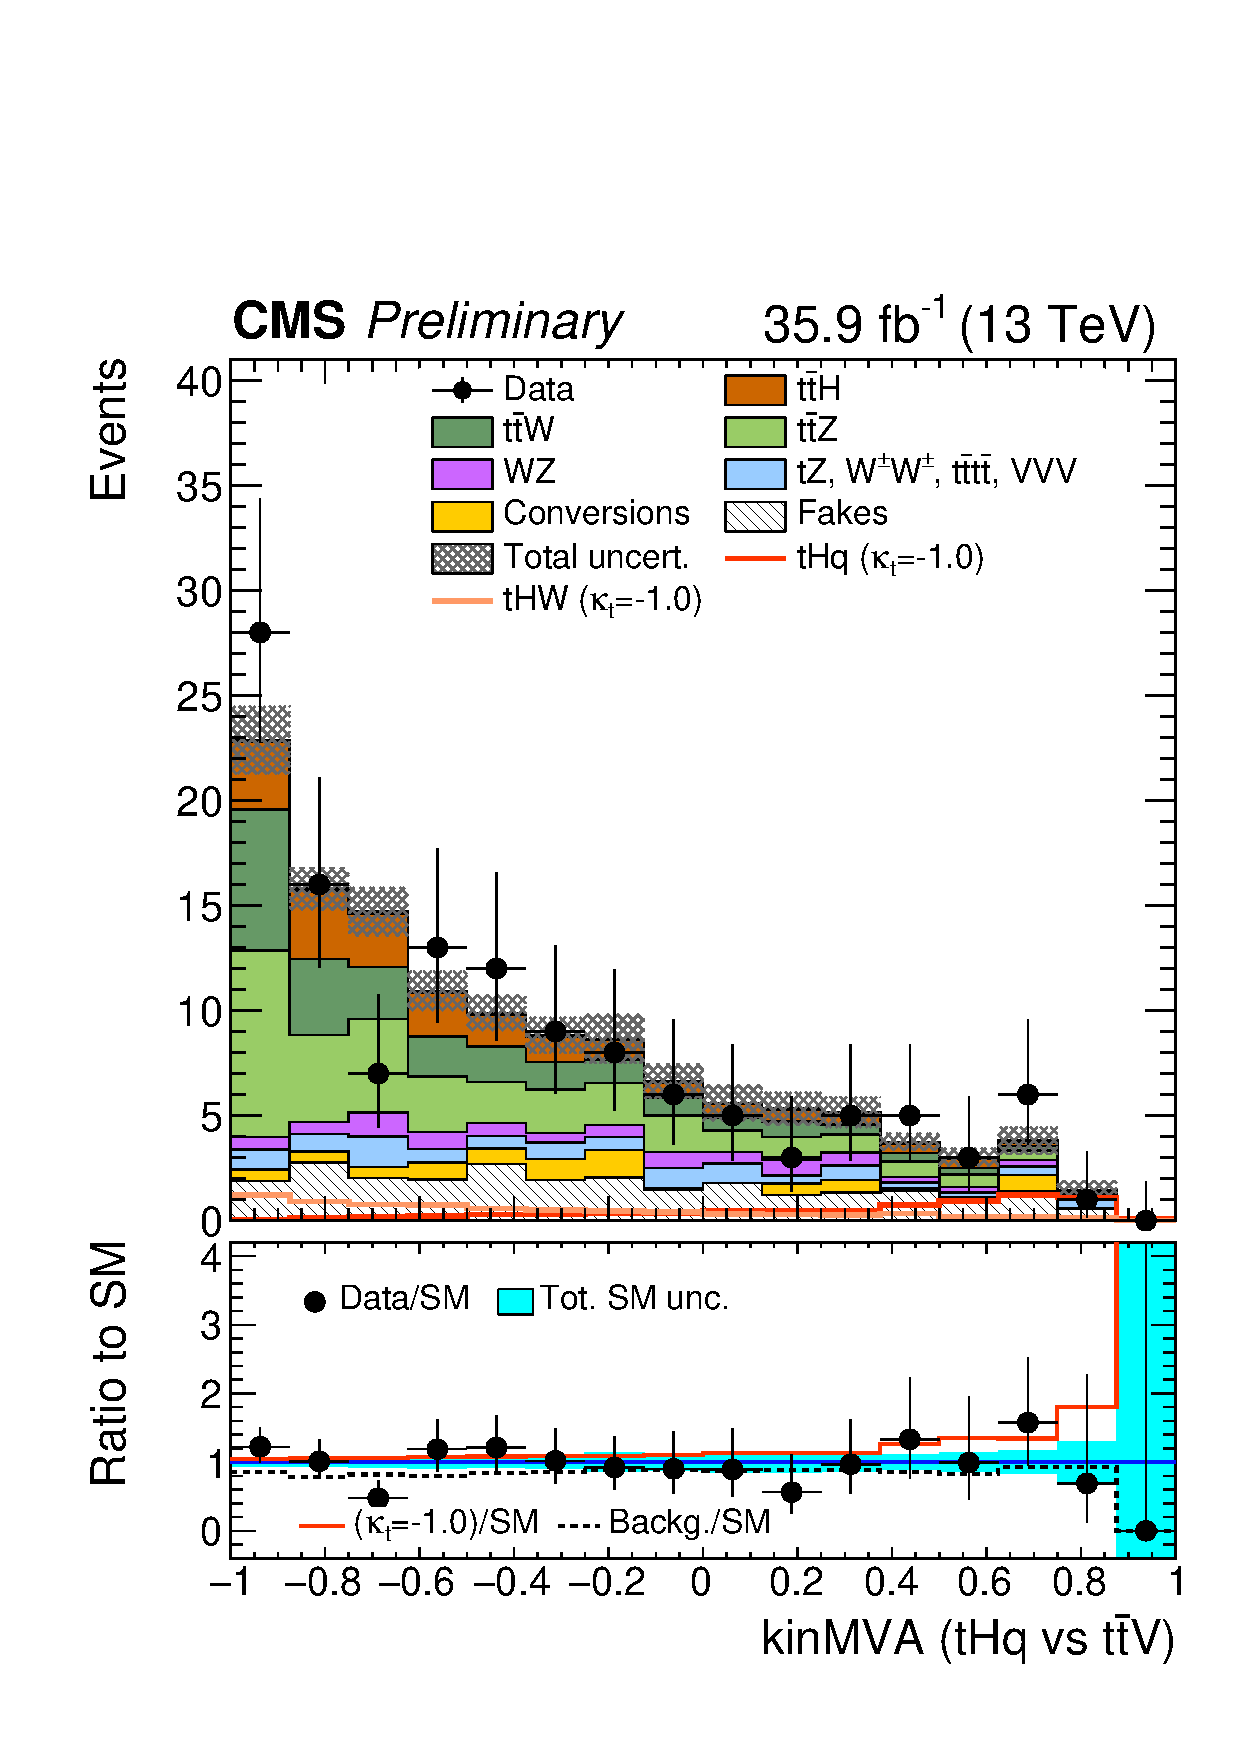
\includegraphics[width=0.32\textwidth]{Figures/polished/thqMVA_ttv_3l_40_3l.pdf} 
    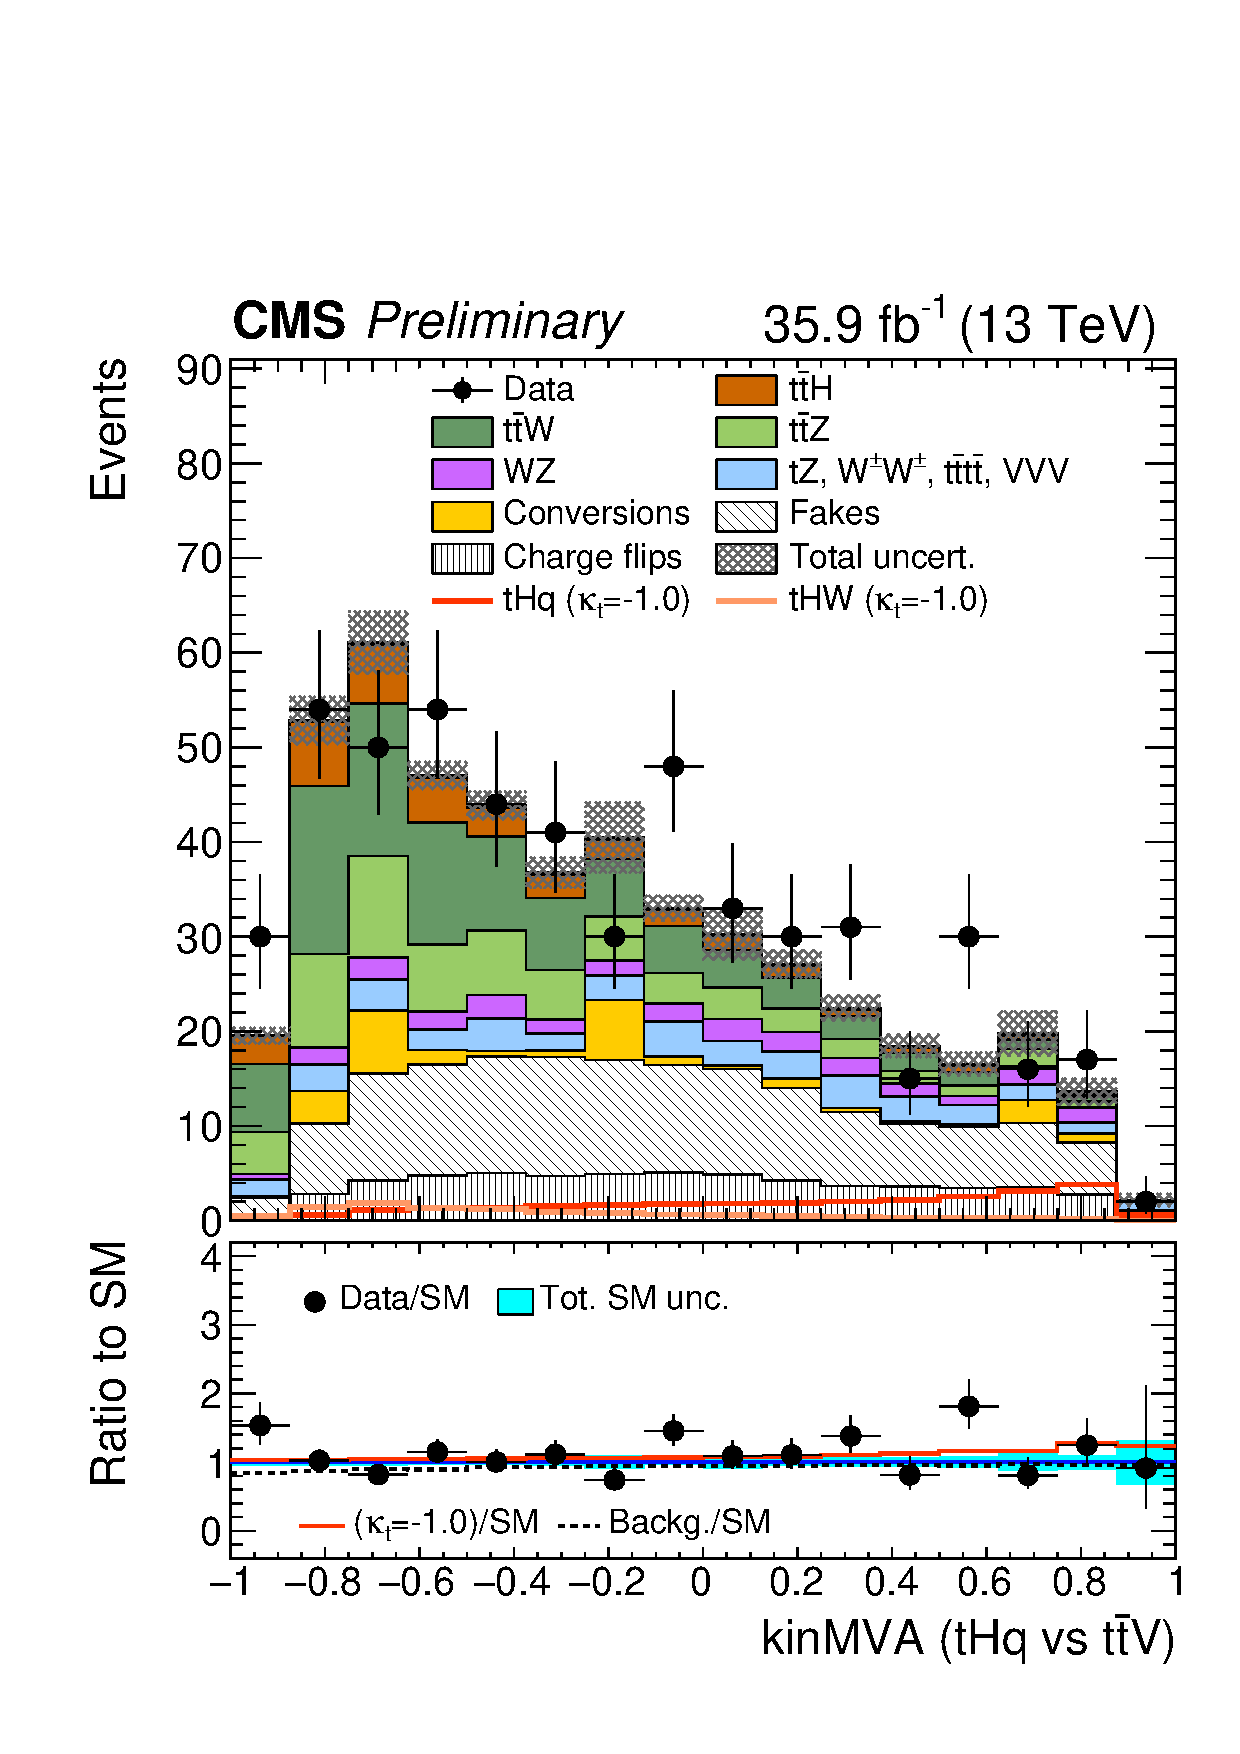
\includegraphics[width=0.32\textwidth]{Figures/polished/thqMVA_ttv_2lss_40_em.pdf}
    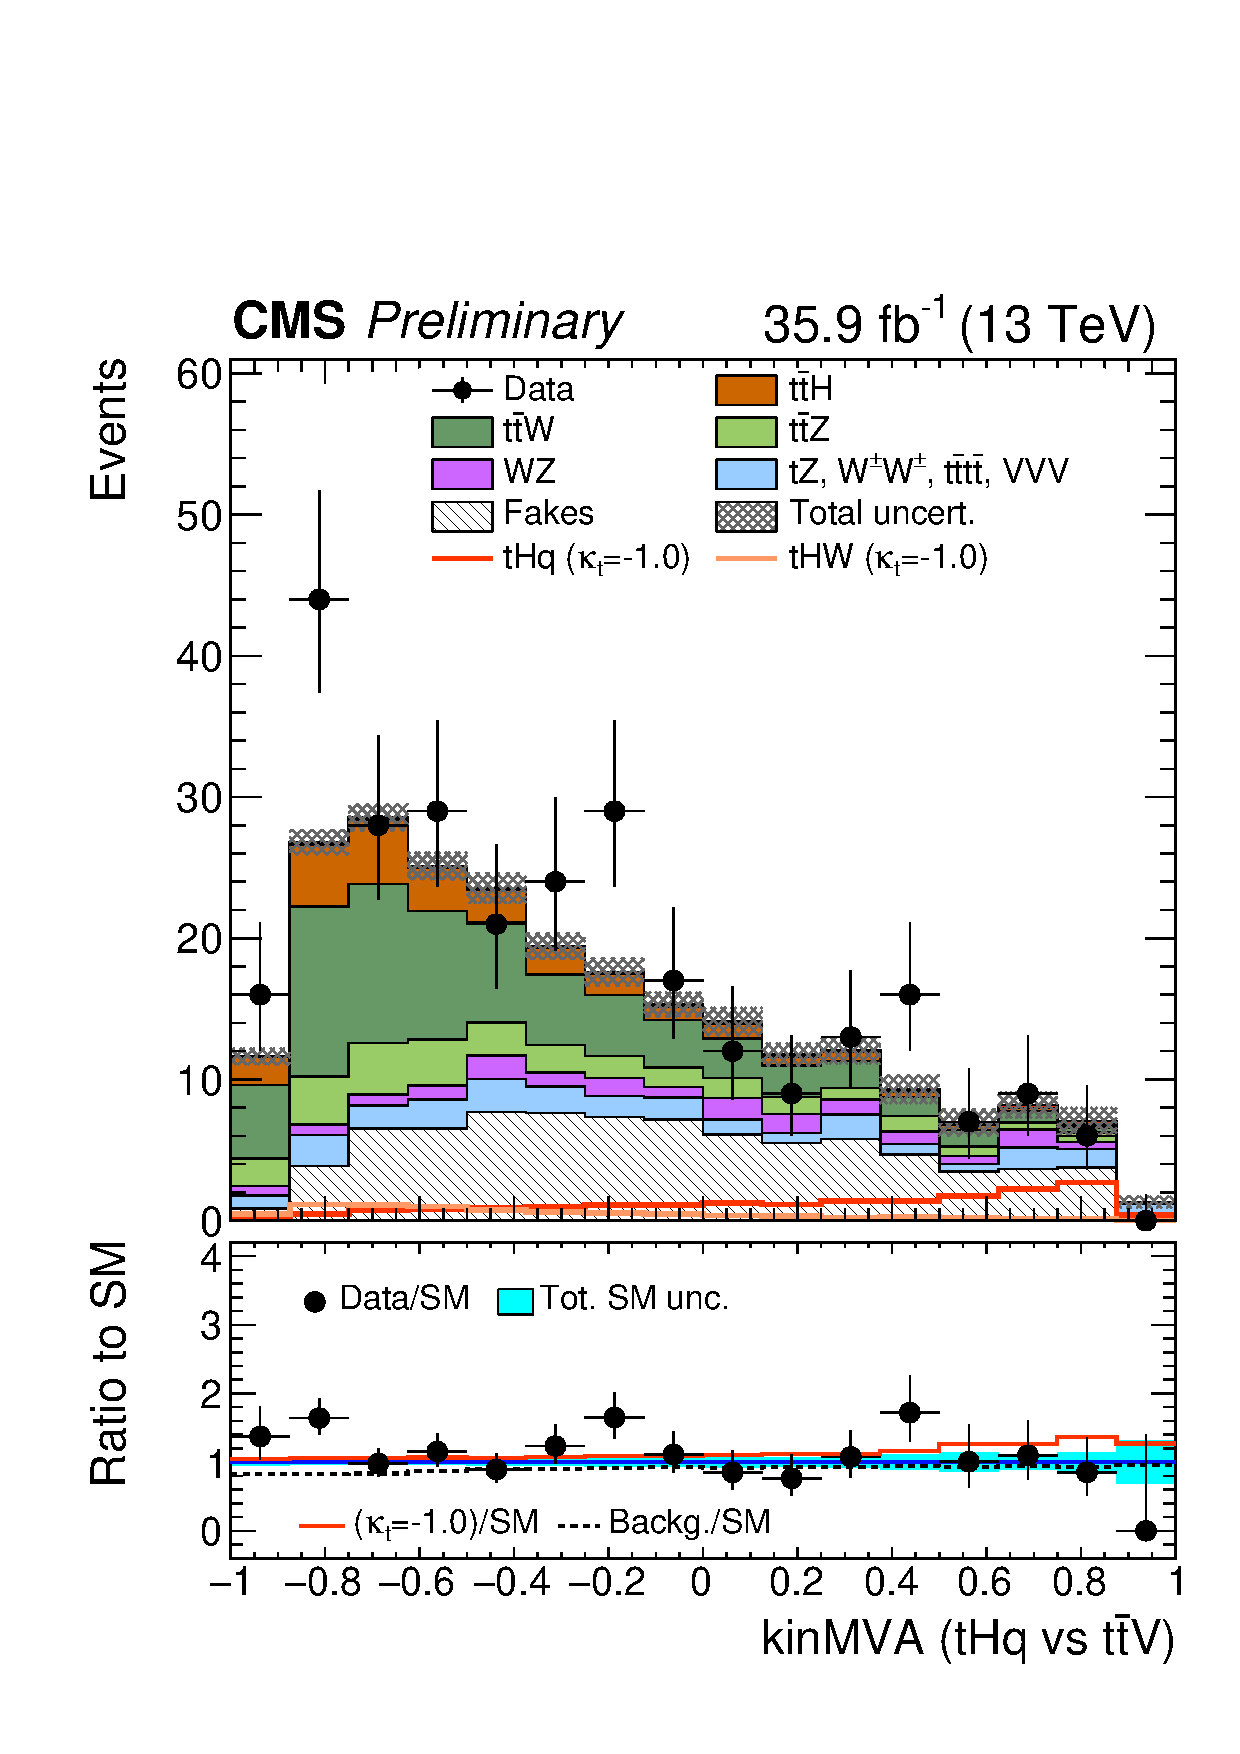
\includegraphics[width=0.32\textwidth]{Figures/polished/thqMVA_ttv_2lss_40_mm.pdf} \\
    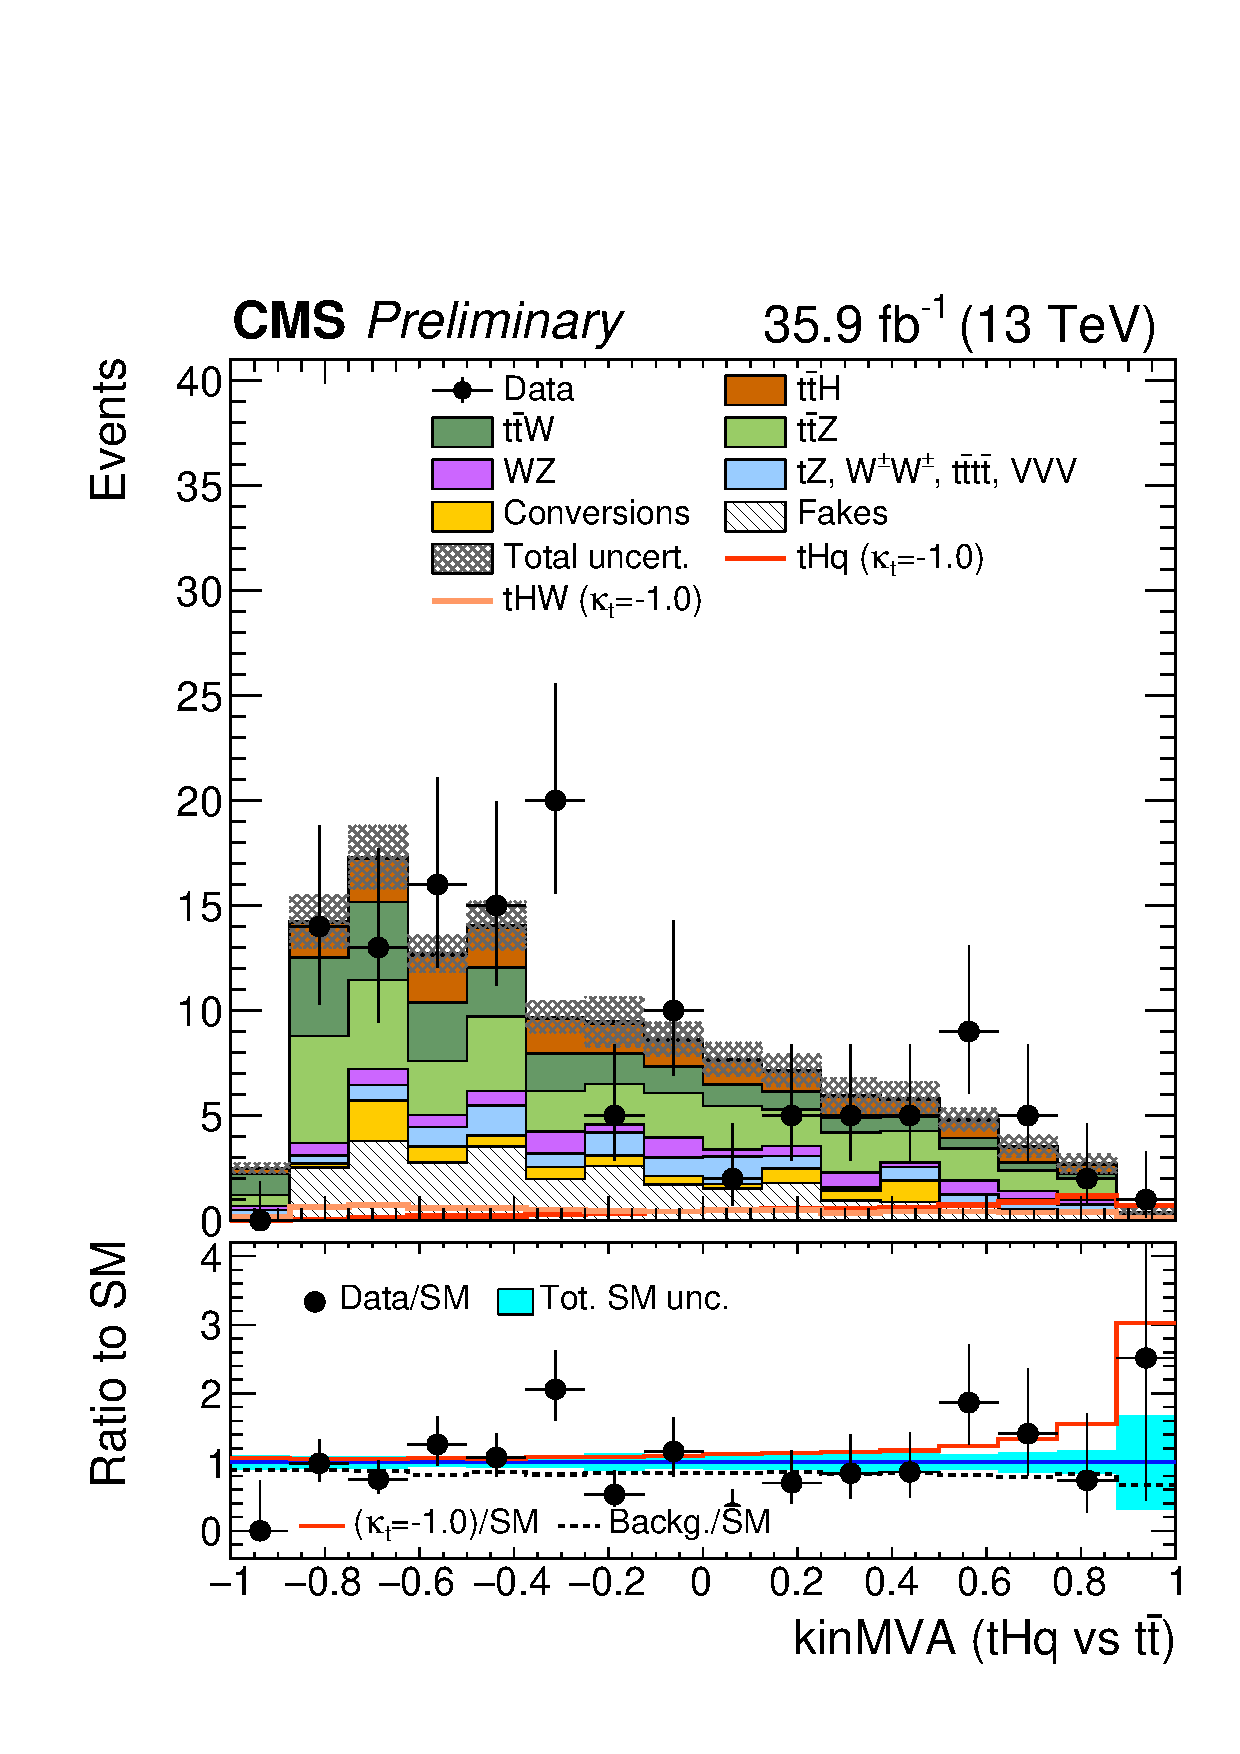
\includegraphics[width=0.32\textwidth]{Figures/polished/thqMVA_tt_3l_40_3l.pdf}
    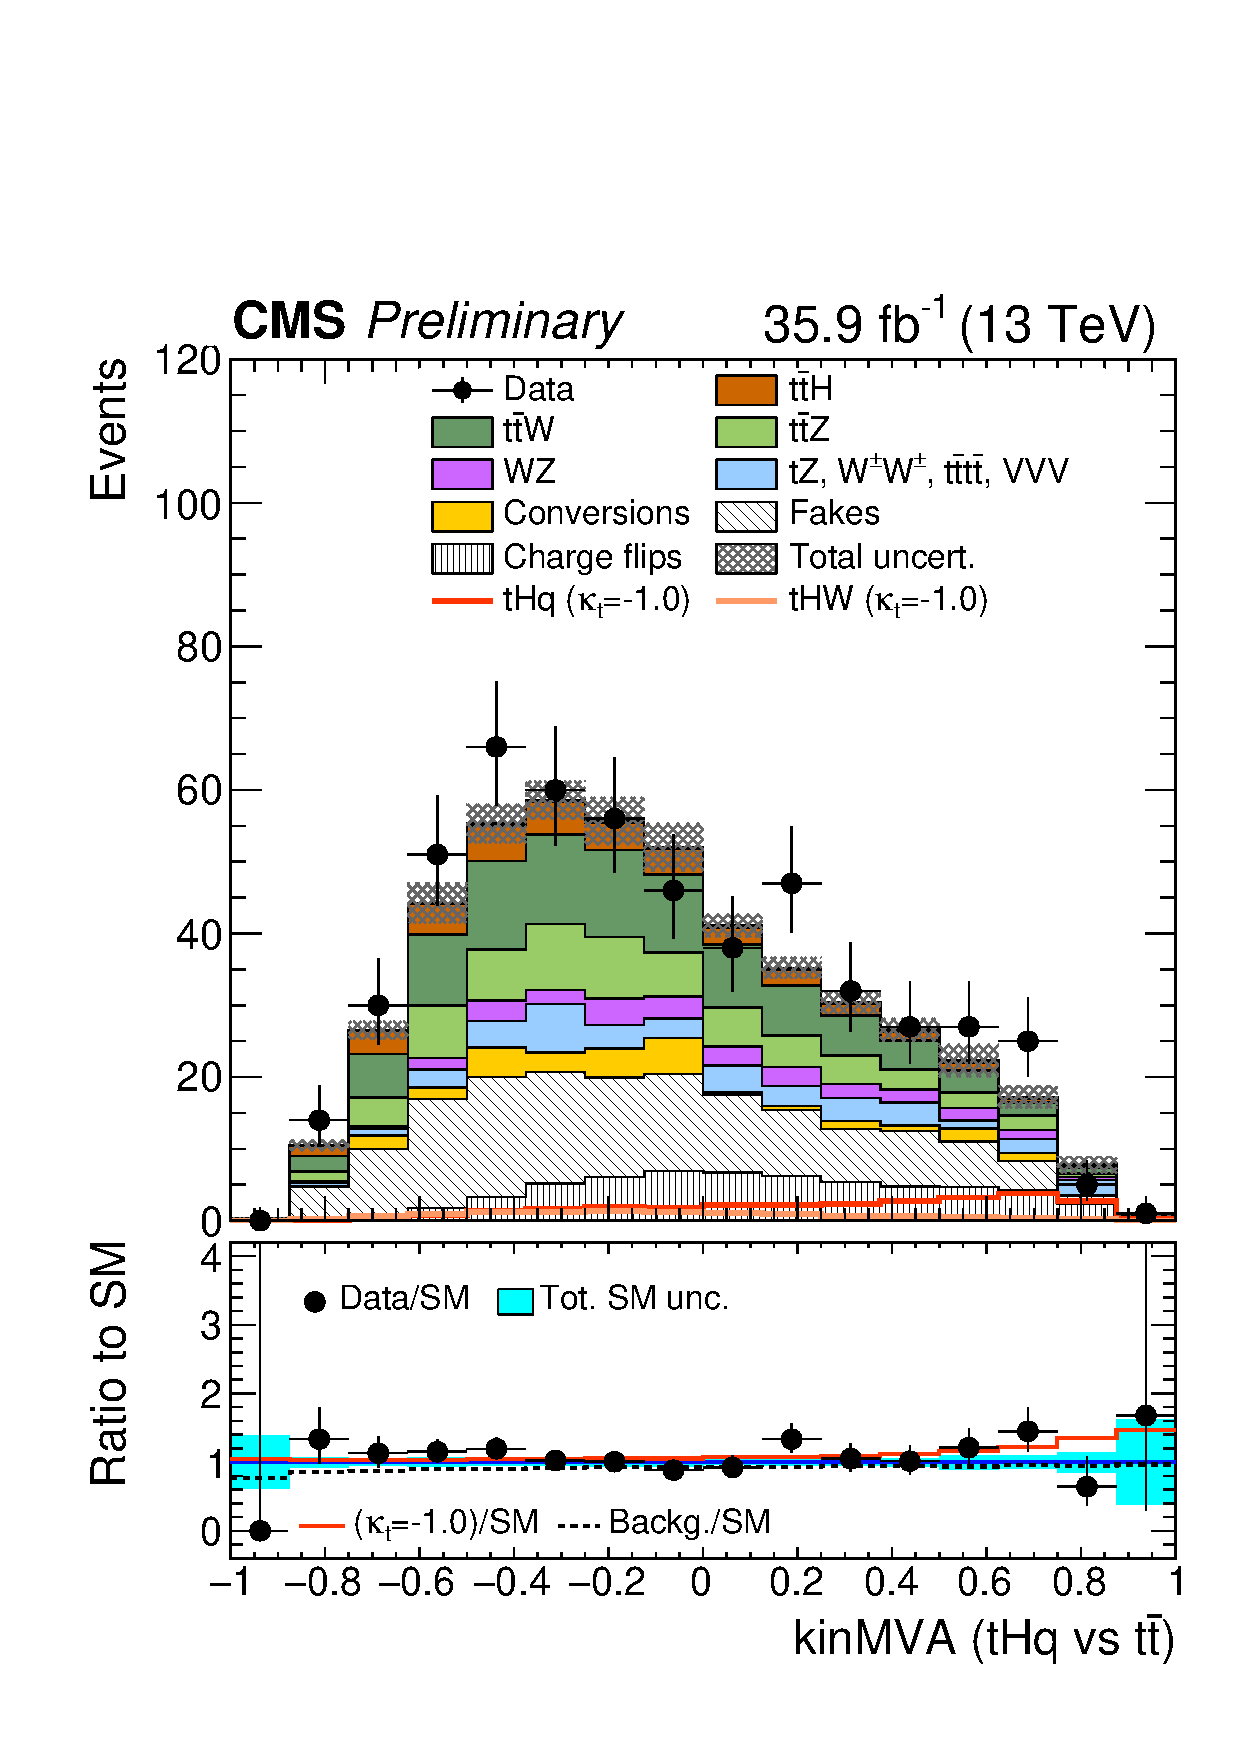
\includegraphics[width=0.32\textwidth]{Figures/polished/thqMVA_tt_2lss_40_em.pdf}
    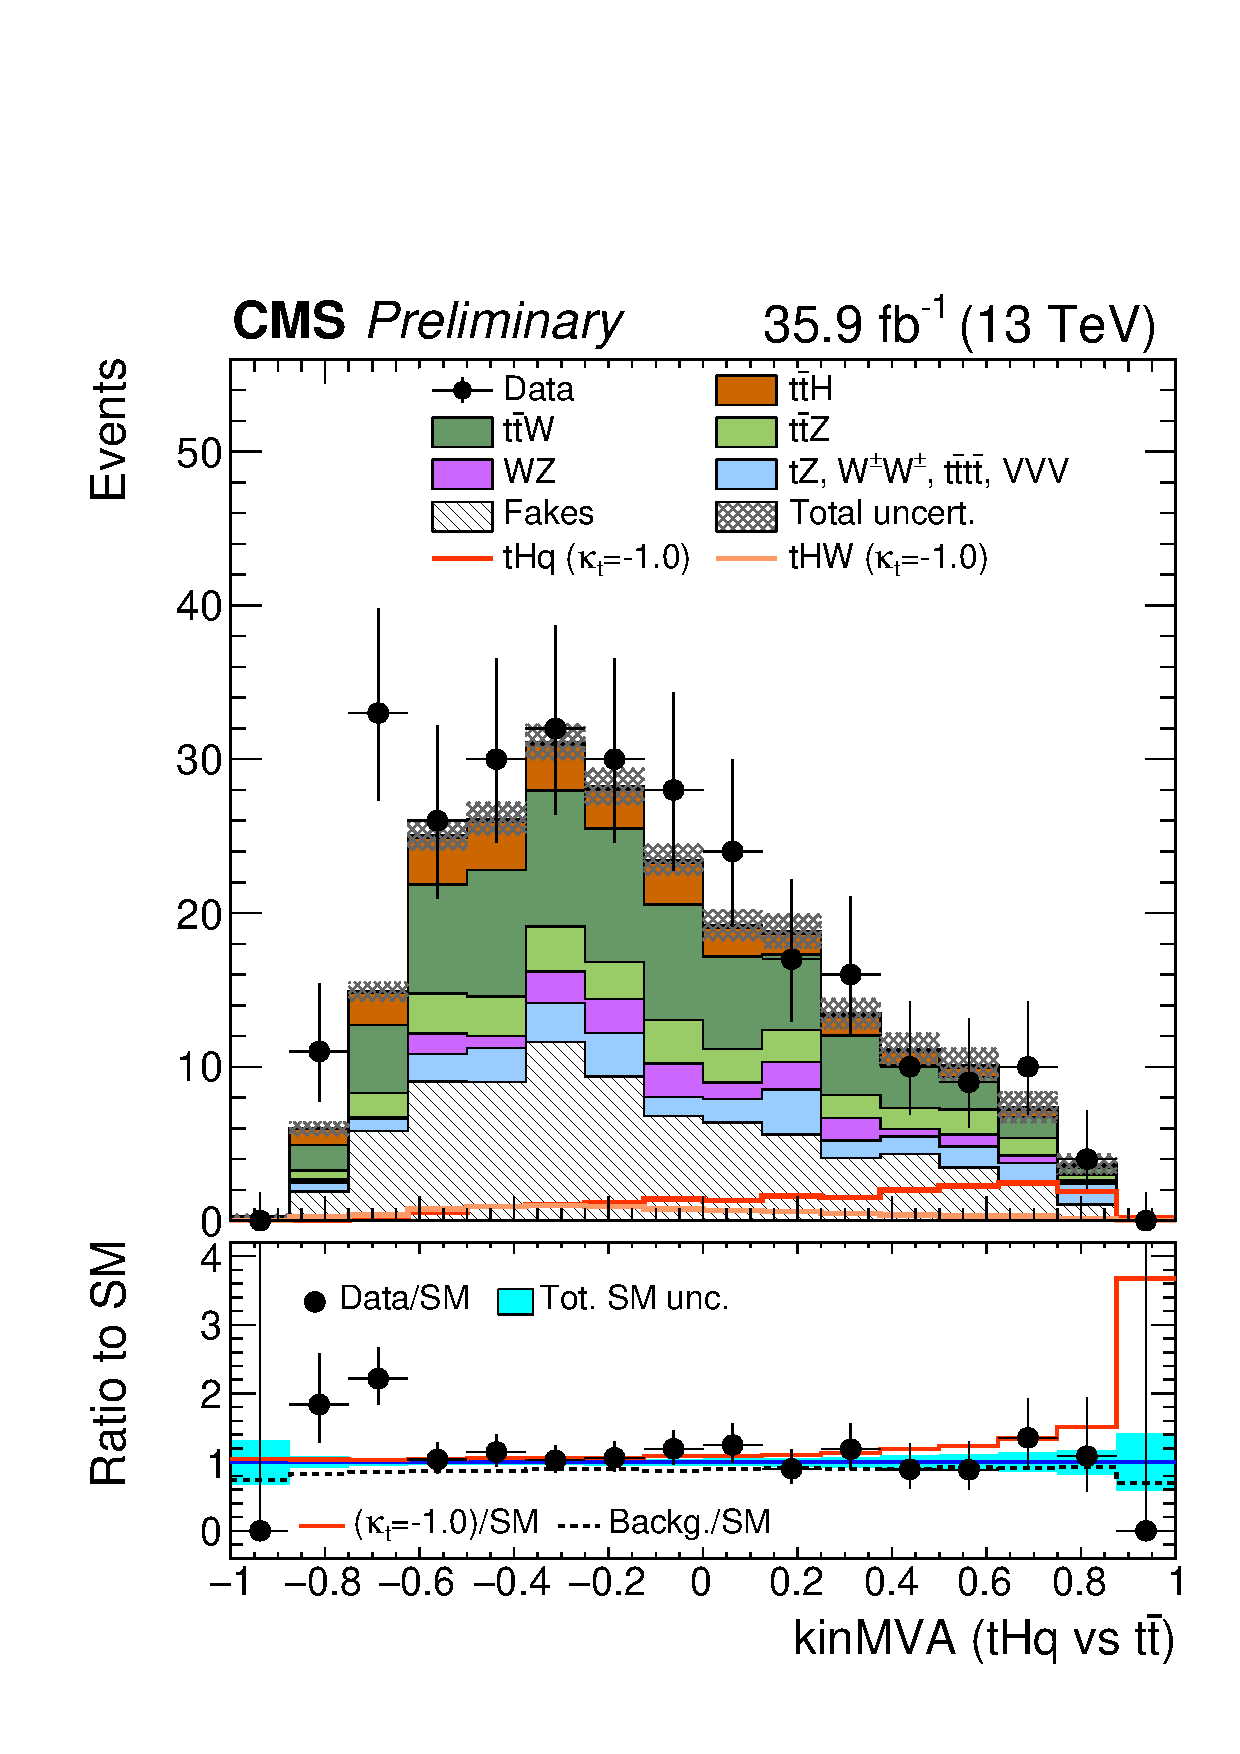
\includegraphics[width=0.32\textwidth]{Figures/polished/thqMVA_tt_2lss_40_mm.pdf}
  \end{center}
  \caption{Pre-fit BDT classifier outputs, for the three-lepton channel (left), \emu\ (center), and \mumu\ (right), for 35.9~\fbinv, for training against \ttV\ (top row) and against \ttbar\ (bottom row).
  In the box below each distribution, the ratio of the observed and predicted event yields is shown.
  The shape of the two \tH\ signals for $\Ct=-1.0$ is shown, normalized to their respective cross sections for $\Ct=-1.0, \CV=1.0$.
  The grey band represents the unconstrained (pre-fit) statistical and systematical uncertainties.\label{fig:postfitshapes}}
\end{figure}

\begin{figure}[!htb]
  \begin{center}
    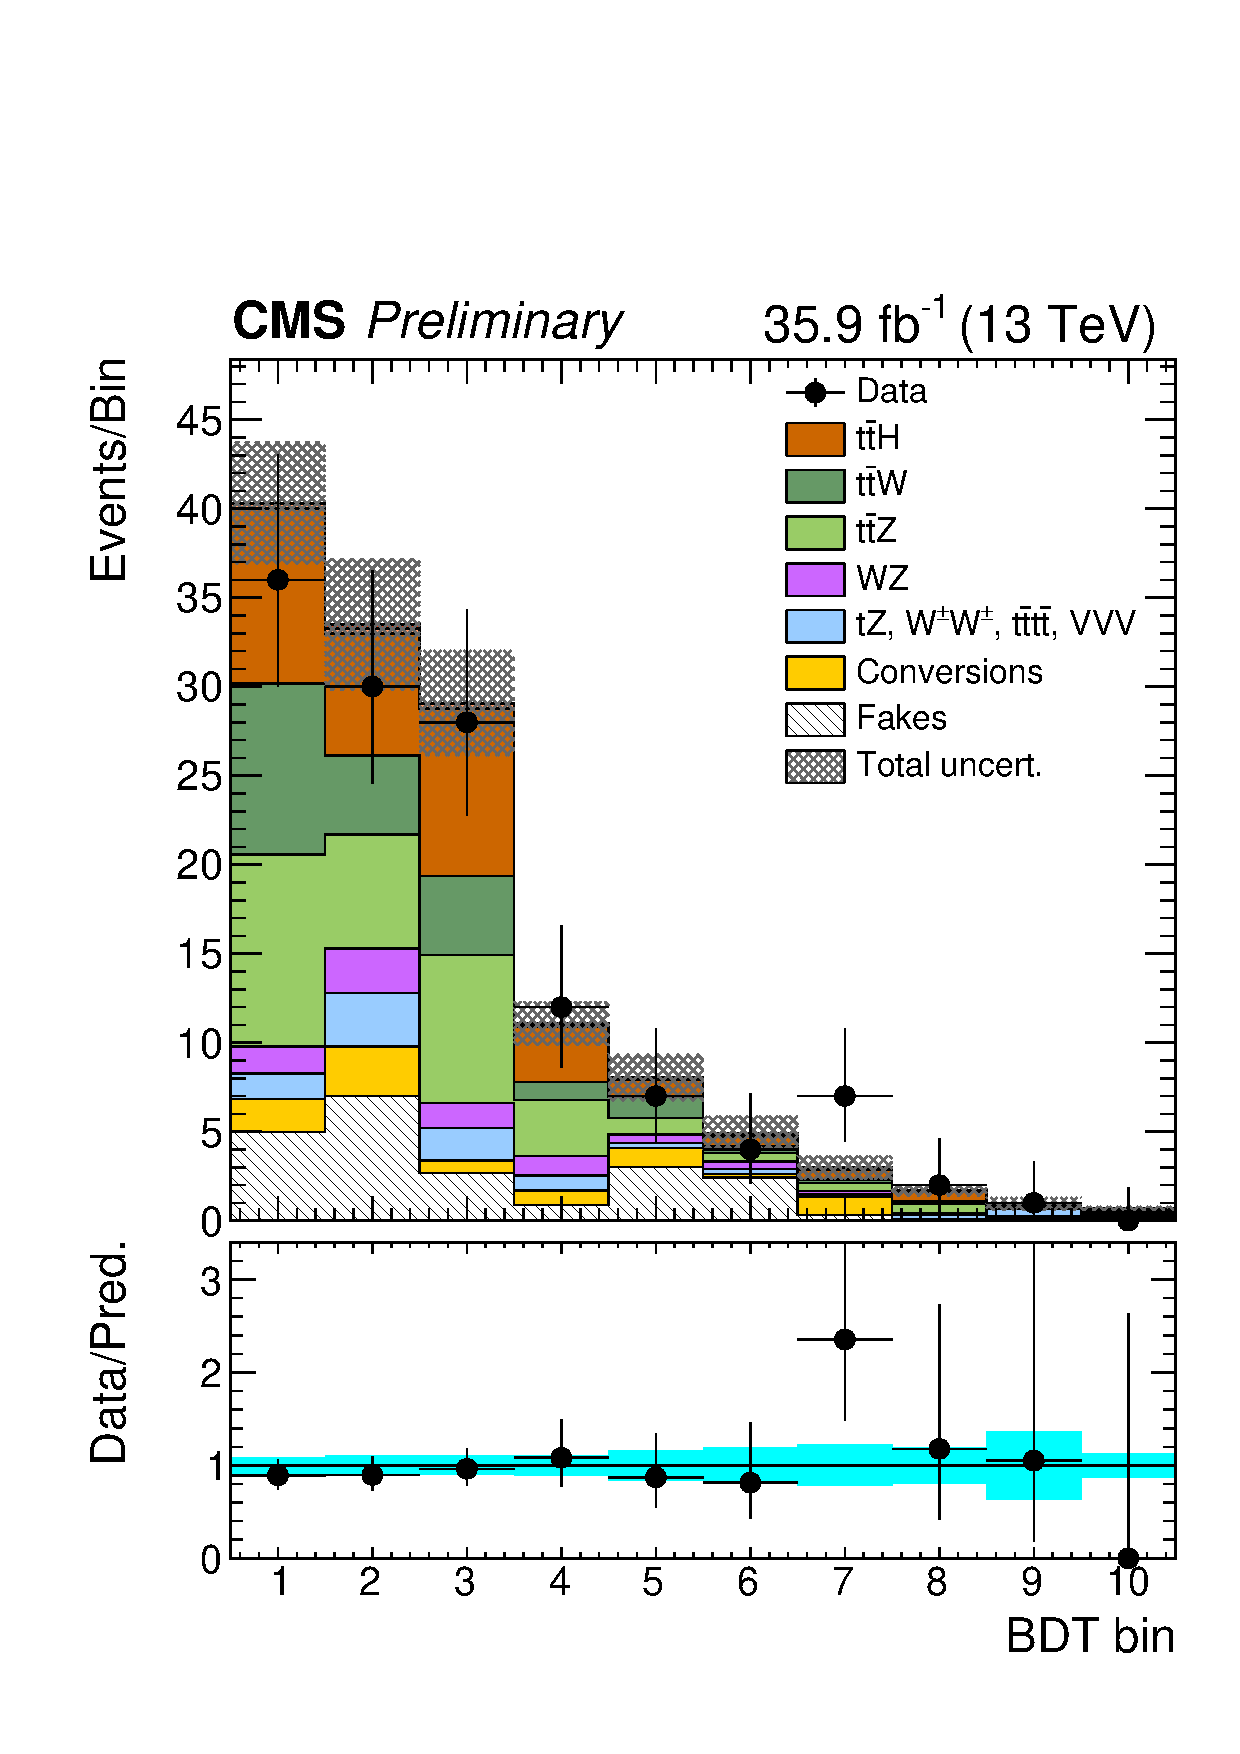
\includegraphics[width=0.32\textwidth]{Figures/postfit/tHq_3l_13TeV_fit_s.pdf}
    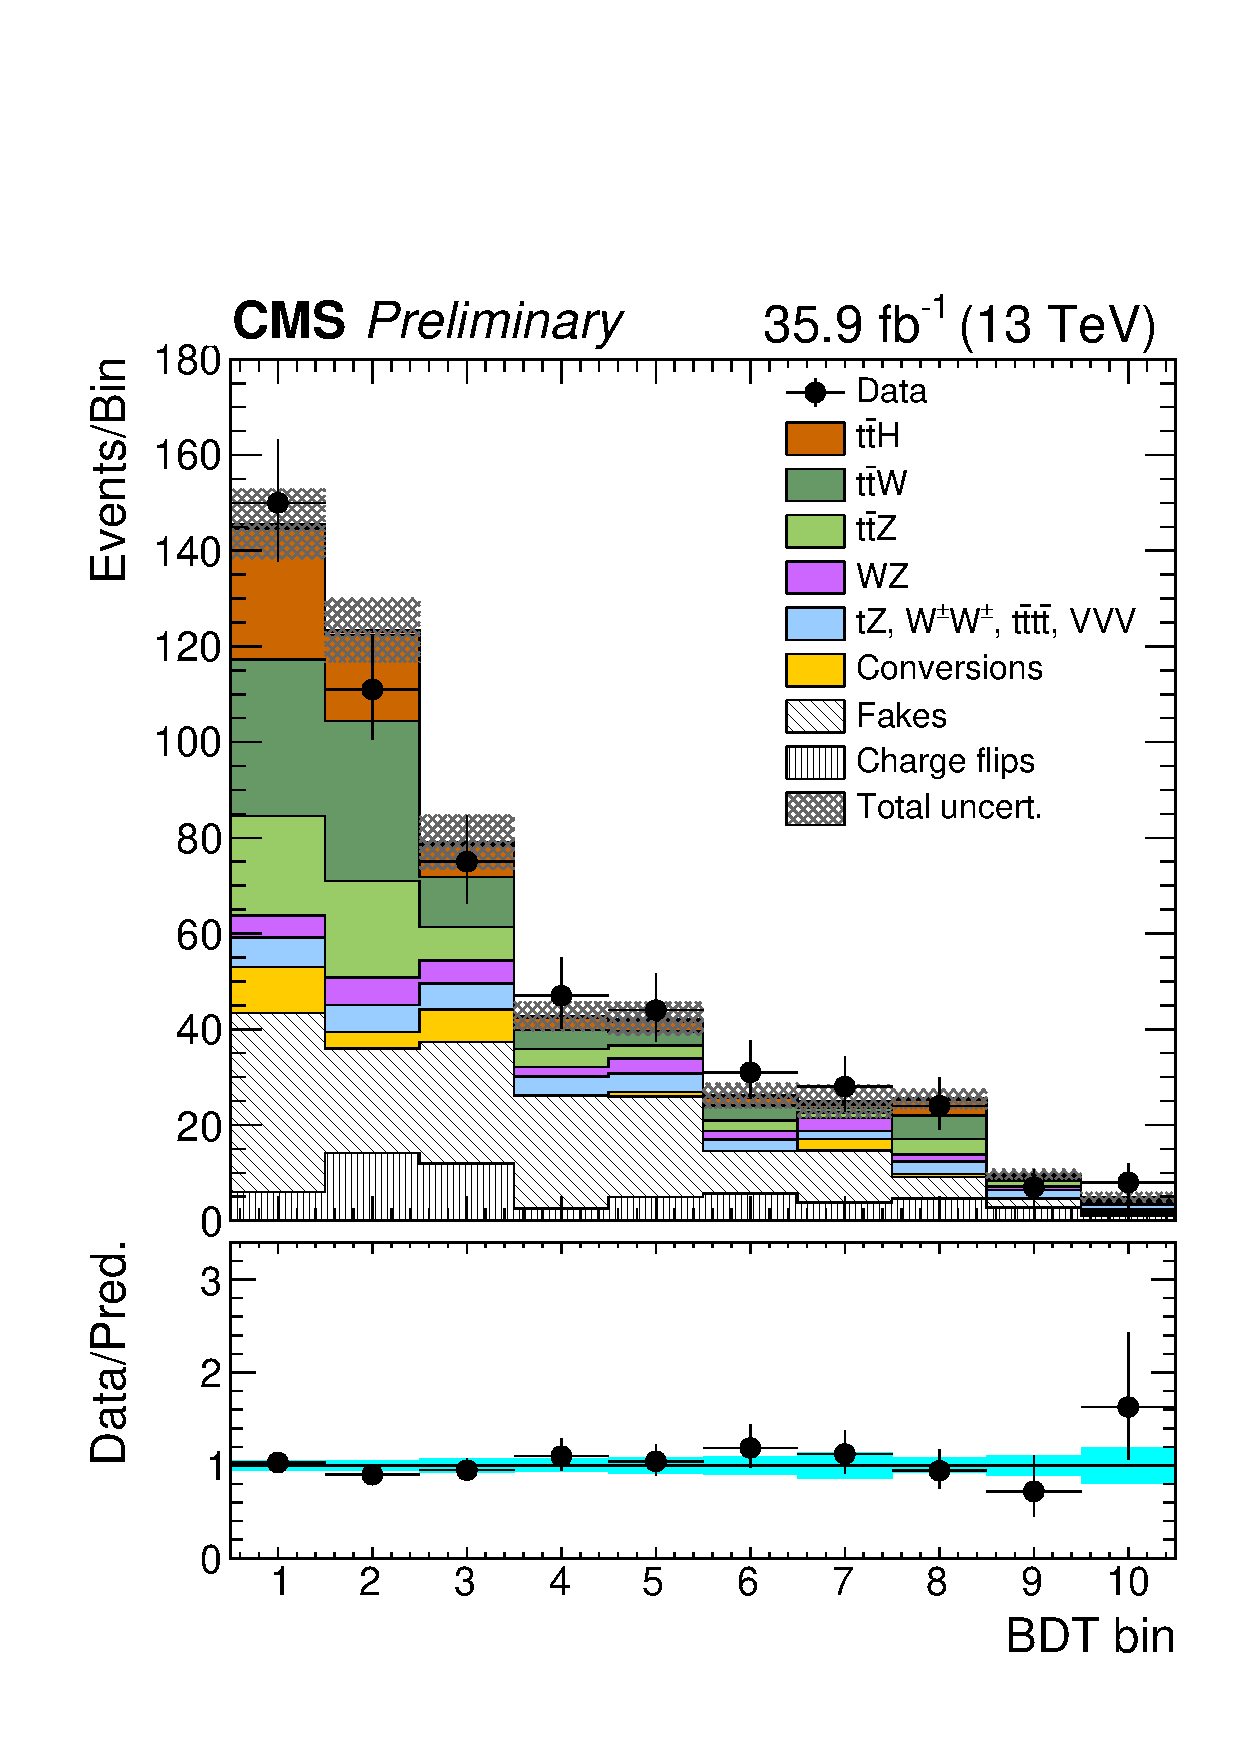
\includegraphics[width=0.32\textwidth]{Figures/postfit/tHq_2lss_em_13TeV_fit_s.pdf} 
    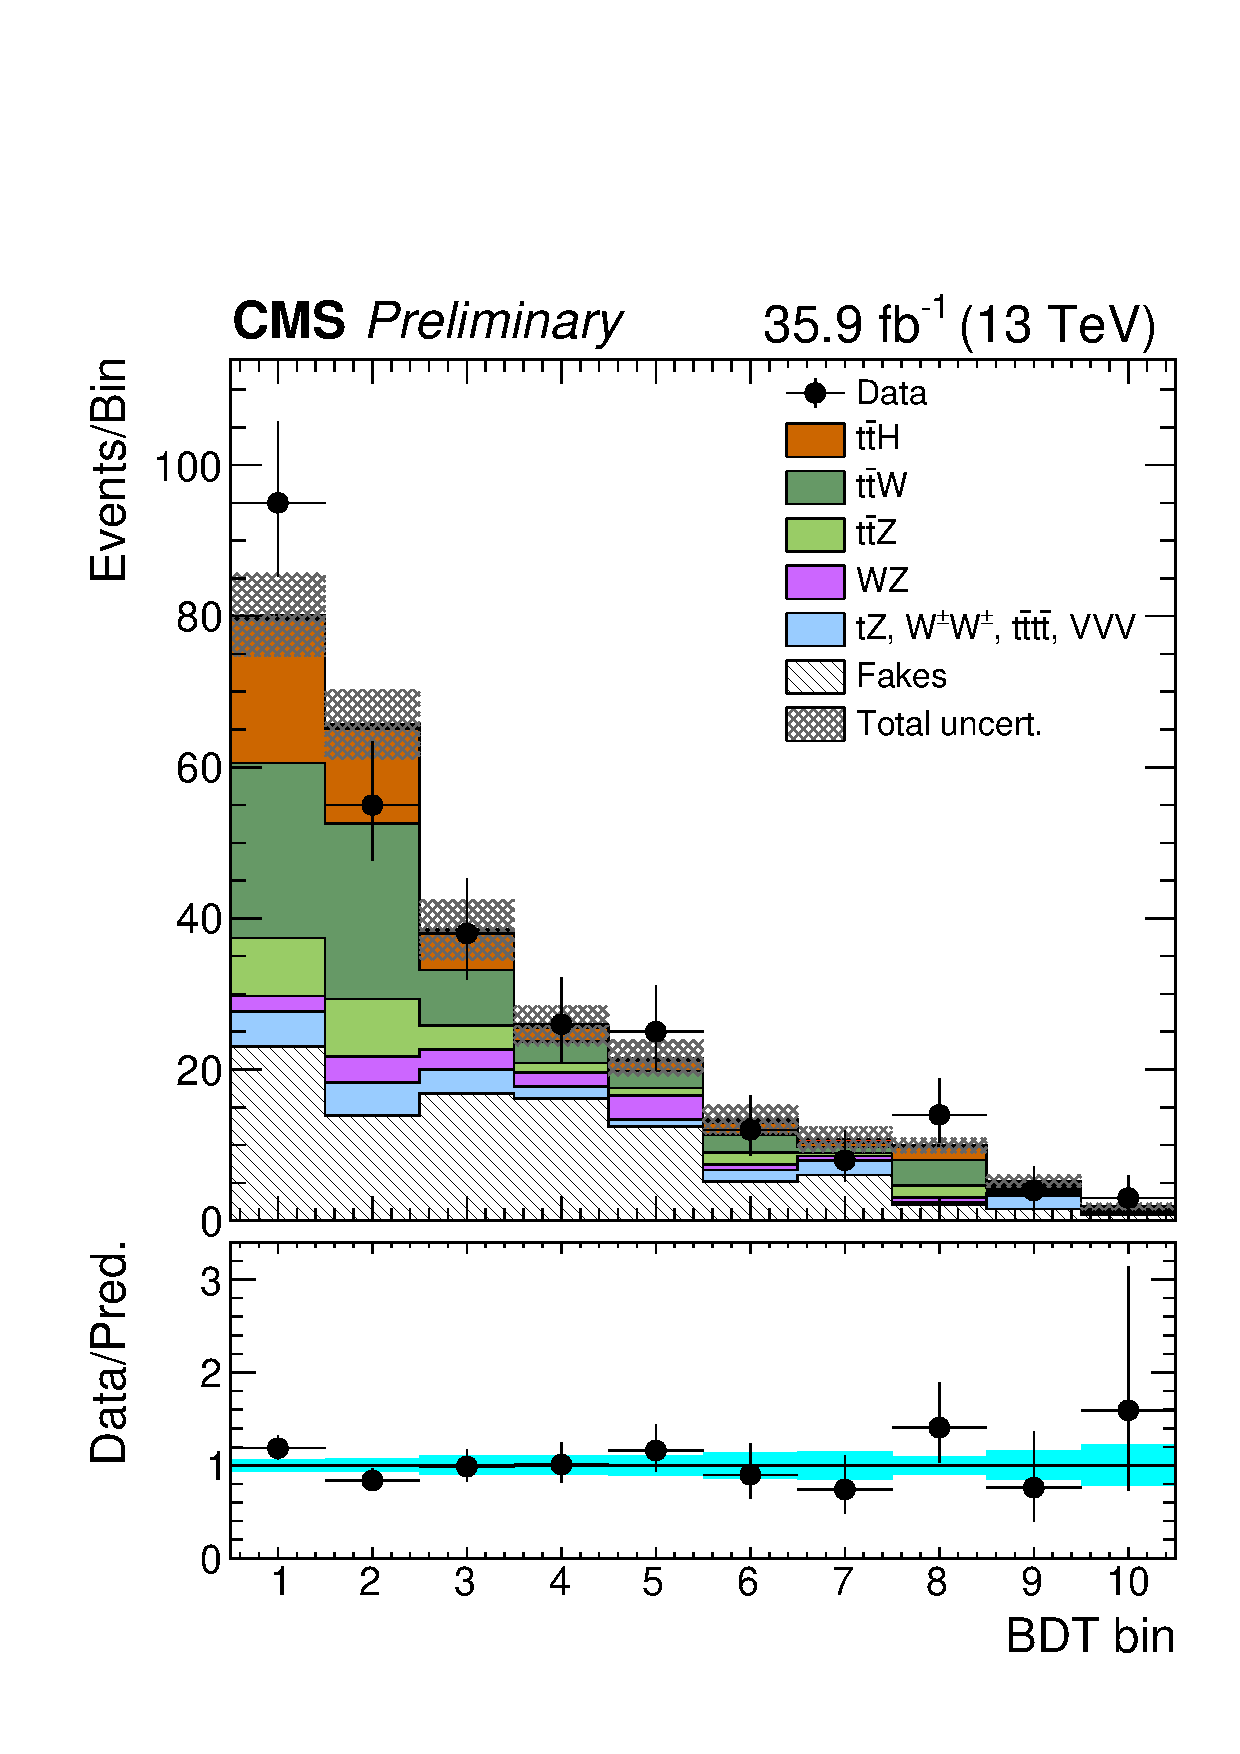
\includegraphics[width=0.32\textwidth]{Figures/postfit/tHq_2lss_mm_13TeV_fit_s.pdf}
  \end{center}
  \caption{Post-fit categorized BDT classifier outputs as used in the maximum likelihood fit for the three-lepton channel (left), \emu\ (center), and \mumu\ (right), for 35.9~\fbinv.
  In the box below each distribution, the ratio of the observed and predicted event yields is shown.
  % The grey band represents the unconstrained (pre-fit) statistical and systematical uncertainties.
  \label{fig:finalbins}}
\end{figure}

The observed 95\% C.L. upper limits on the $\tH+\ttH$ signal cross sections for the case of inverted couplings ($\Ct/\CV=-1.0$) for the individual channels are, respectively, $1.00$, $0.84$, and $0.70\,\mathrm{pb}$ for the \mumu, \emu, and trilepton final states, corresponding to $2.3$, $1.9$, and $1.6$ times the respective expected cross sections for $\CV=1.0$.
The combination of all three channels yields a limit of $0.64\,\mathrm{pb}$ on a signal shape expected for $\Ct/\CV=-1.0$, corresponding to $1.4$ times the expected $\tH+\ttH$ cross section with $\Ct=-1.0, \CV=1.0$.
% In this evaluation, all extra Higgs boson yields arising from the $\Ct=-1$ condition are considered as signal.
In the standard model scenario ($\Ct/\CV=1.0$), the observed upper limit on the cross section times branching ratio is $0.56\,\mathrm{pb}$, corresponding to $3.1$ times the expected SM cross section of $\tH+\ttH$.
Table~\ref{tab:limits} summarizes the results for the inverted coupling scenario and for the standard model.

The best-fit combined signal strength for the standard model hypothesis is $1.8\,\pm\,0.3\mathrm{(stat.)}\,\pm\,0.6\mathrm{(syst.)}$, corresponding to an observed significance of $2.7\sigma$ ($1.5\sigma$ expected) over a background-only hypothesis.
For a scenario of inverted couplings ($\Ct=-1=-\CV$), the best fit signal strength is $0.7\pm0.4$, corresponding to a significance of $1.7\sigma$ ($2.5\sigma$ expected), whereas the fit prefers a signal strength compatible with $0$ for a scenario with $\Ct=0$ (where the \ttH\ component vanishes).

The expected and observed limits are shown in Fig.~\ref{fig:limits} as a function of $\Ct/\CV$. %  and their 68\% and 95\% C.L. uncertainty ranges,
Comparing the observed upper limit with the theoretical prediction of the $\tH+\ttH$ cross section times BR for $\CV=1.0$ constrains the allowed range of coupling configurations $\Ct/\CV$ to between about $-1.25$ and $+1.60$.

\begin{table}[h!]
  \begin{center}
    \begin{tabular}{llcccc} \hline 
      Scenario  & Channel  & Obs. Limit    & \multicolumn{3}{c}{Exp. Limit (pb)}         \\
                &          & (pb)          & Median        & $\pm1\sigma$ & $\pm2\sigma$ \\ \hline \hline
   $\Ct/\CV=-1$ & \mumu\   & 1.00          &         0.58  & [0.42, 0.83] & [0.31, 1.15] \\
                & \emu\    & 0.84          &         0.54  & [0.39, 0.76] & [0.29, 1.03] \\
                & \threel\ & 0.70          &         0.38  & [0.26, 0.56] & [0.19, 0.79] \\ 
                & Combined & \textbf{0.64} & \textbf{0.32} & [0.22, 0.46] & [0.16, 0.64] \\ \hline
    $\Ct/\CV=1$ & \mumu\   & 0.87          &         0.41  & [0.29, 0.58] & [0.22, 0.82] \\
    (SM-like)   & \emu\    & 0.59          &         0.37  & [0.26, 0.53] & [0.20, 0.73] \\
                & \threel\ & 0.54          &         0.31  & [0.22, 0.43] & [0.16, 0.62] \\
                & Combined & \textbf{0.56} & \textbf{0.24} & [0.17, 0.35] & [0.13, 0.49] \\ \hline
    \end{tabular}
    \caption{Expected and observed 95\% C.L. upper limits on the $\tH+\ttH$ production cross section times $\PH\to\W\W^*+\tautau+\Z\Z^*$ branching ratio for a scenario of inverted couplings ($\Ct/\CV=-1.0$, top rows) and for a standard-model-like signal ($\Ct/\CV=1.0$, bottom rows), in pb. The expected limit is calculated on a background-only MC dataset. % and quoted with $\pm$1$\sigma$ and $\pm$2$\sigma$ probability ranges.
    \label{tab:limits}}
  \end{center}
\end{table}

\begin{figure}[!h]
  \centering
  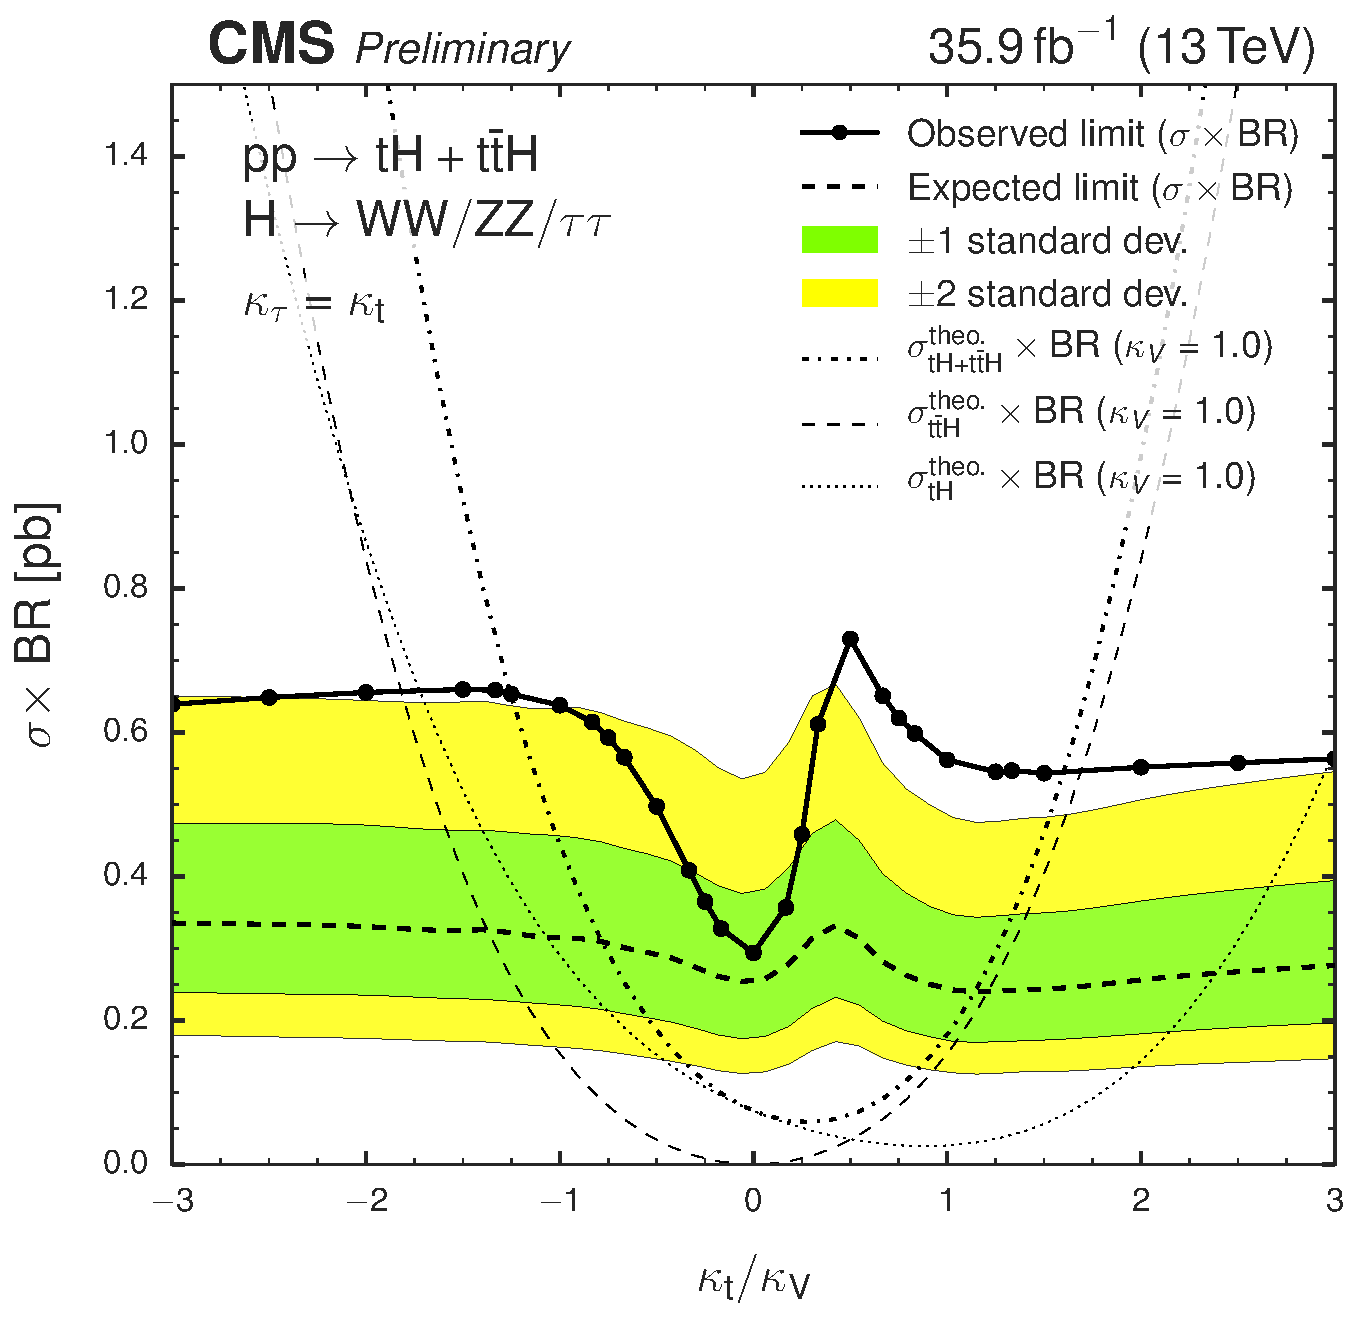
\includegraphics[width=0.8\textwidth]{Figures/xs_limits_K6.pdf}
  \caption{Observed and expected 95\% C.L. upper limit on the $\tH+\ttH$ cross section times $\PH\to\W\W^*+\tautau+\Z\Z^*$ branching fraction for different values of the coupling ratio \Ct/\CV. The expected limit is derived from a background-only MC dataset. % and shown with its $\pm1\sigma$~(green) and $\pm2\sigma$~(yellow) probability bands.
  \label{fig:limits}}
\end{figure}

The sensitivity of the analysis is limited by systematic uncertainties, predominantly by those concerning the normalizations of the main background components (the non-prompt lepton estimation, the scale uncertainties for $\ttW$ and $\ttZ$), as well as by the uncertainties on the measured lepton efficiency.


% Conclusions
\hyphenation{diffe-rent}
%%%%%%%%%%%%%%%%%%%%% Conclusions %%%%%%%%%%%%%%%%%
\chapter{CONCLUSIONS}
\label{ch:Conclusions}

\hspace{1cm} Metal/semiconductor interface formation was studied by X-ray photoemission spectroscopy. It was found that boron carbide-based semiconductors behave different from other semiconductor materials, since it presents Schottky barrier formation when working with p-type heterojunctions. Being the work function of the gold, the metal used for this study, bigger than this for the semiconductor, it is expected to see signatures of omhic contacts in the interface between the metal and the semiconductor, i.e., binding energies shifting to small values, or not change in the binding energy. However, shifting of the binding energies for the B(1s) and C(1s) core levels to high energies was found, can be explained by having a Schottky barrier formation in the interface.  The opposite situation is found when working with n-type boron carbide semiconductors and gold. No band bending signatures were found, therefore an ohmic contact is assigned to this surface interaction, confirming the unusual behavior of these heterojunctions. Inclusion of the aromatic compunds aniline seems to increase the Schottky barrier formed on the interface in the case of p-type heterojunctions. \\ 

\noindent \hspace{1cm} From electrical and optical measurements on these boron carbide-based heterojunctions, it was found that semiconducting boron carbides exhibit significantly enhanced electron-hole separation with inclusion of the aromatic compounds. For the case of \textit{ortho}-carborane boron carbide films, carrier lifetimes increase from 35 $\mu s$, for the pure boron carbide, to 350 $\mu s$ with pyridine inclusion, and even better to 2.5 $ms$ with benzene inclusion. The findings of substantially enhanced electron-hole separation and carrier lifetime in the doped films versus pure boron carbide films are certainly encouraging for the application of these materials as solid state neutron detectors. \\

\noindent \hspace{1cm} In the case of the addition of pyridine linking groups to PECVD semiconducting hydrogenated boron carbide films, synthesized on n-type silicon, it was found that charge collection increases, after neutron capture, in a heterojunction diode with silicon at zero bias, and the charge collection is much improved compared to heterojunction diodes fabricated by PECVD but without pyridine. The spatial overlap of the HOMO and LUMO states in cluster calculations, if applicable to the solid, suggests that exciton decay is facile, but hindered by symmetry constraints. \\ %(J. Phys. D: Appl. Phys. 49 355302)


\noindent \hspace{1cm} Finally, it was shown that semiconducting boron carbide polymers, formed by site-specific cross-linking of orthocarborane icosahedra with and without 1,4 diaminobenzene, exhibit significant negative magnetoresistive effect at room temperature. Values over 450\% negative magnetoresistance, depending on the bias voltage, are found for the pure boron carbide, while for samples with diaminobenzene doping it was about 100\%. Although inclusion of diaminobenzene does not improve the negative magnetoresistance values, other aromatic compounds need to be tested to determine whatever or not doping will affect the magnetoresistance of the films.  




%% **DO NOT REMOVE BIBLIOGRAPHY**
\clearpage\newpage
\bibliography{auto_generated}   % will be created by the tdr script.

%%%%%%%%%%%%%%%
\end{document}


